\documentclass[12pt,a4paper]{article}

% ==============================================================================
% PAQUETES BÁSICOS Y CODIFICACIÓN
% ==============================================================================
\usepackage[T1]{fontenc}
\usepackage[utf8]{inputenc}
\usepackage[spanish,es-tabla,es-noquoting]{babel}

% Márgenes idénticos al documento Word original (2.3 cm laterales, 2.0 cm sup/inf)
\usepackage[a4paper, left=2.3cm, right=2.3cm, top=2.0cm, bottom=2.0cm]{geometry}

% Fuente Calibri idéntica a Word mediante la tipografía Carlito
\usepackage{carlito}
\renewcommand{\familydefault}{\sfdefault}

% Paquetes para tablas, gráficos y diseño
\usepackage{graphicx}
\usepackage{array}
\usepackage{tabularx}
\usepackage{booktabs}
\usepackage{amsmath,amssymb}
\usepackage{float}
\usepackage{caption}
\usepackage{subcaption}
\usepackage{xcolor}
\usepackage{listings}
\usepackage{enumitem}
\setlist{itemsep=2.5pt, topsep=3pt, parsep=0pt}
\usepackage[hidelinks]{hyperref}

% Rutas de búsqueda de imágenes
\graphicspath{{img/}{logos/}{./}}

% ==============================================================================
% CONFIGURACIÓN DE CÓDIGO FUENTE
% ==============================================================================
\definecolor{codegreen}{rgb}{0,0.55,0}
\definecolor{codegray}{rgb}{0.45,0.45,0.45}
\definecolor{codepurple}{rgb}{0.55,0,0.8}
\definecolor{backcolour}{rgb}{0.97,0.97,0.97}

\lstdefinestyle{estilocodigo}{
    backgroundcolor=\color{backcolour},   
    commentstyle=\color{codegreen},
    keywordstyle=\color{blue}\bfseries,
    numberstyle=\tiny\color{codegray},
    stringstyle=\color{codepurple},
    basicstyle=\ttfamily\scriptsize,
    breakatwhitespace=false,         
    breaklines=true,                 
    captionpos=b,                    
    keepspaces=true,                 
    numbers=left,                    
    numbersep=6pt,                  
    showspaces=false,                
    showstringspaces=false,
    showtabs=false,                  
    tabsize=2,
    frame=single,
    rulecolor=\color{codegray!40},
    literate={á}{{\'a}}1 {é}{{\'e}}1 {í}{{\'i}}1 {ó}{{\'o}}1 {ú}{{\'u}}1 {ñ}{{\~n}}1 {Á}{{\'A}}1 {É}{{\'E}}1 {Í}{{\'I}}1 {Ó}{{\'O}}1 {Ú}{{\'U}}1 {Ñ}{{\~N}}1
}
\lstset{style=estilocodigo}

% ==============================================================================
% DEFINICIÓN DE MACROS Y FORMATO DE ENCABEZADOS << SECCIÓN >>
% ==============================================================================
\newcommand{\llav}{\symbol{60}\symbol{60}}
\newcommand{\rlav}{\symbol{62}\symbol{62}}
\newcommand{\marcador}[1]{\llav\ #1\ \rlav}
\newcommand{\marcadornospace}[1]{\llav#1\rlav}

% Comando de sección al estilo exacto del Word original
\newcommand{\seccion}[1]{%
  \vspace{0.6cm}%
  {\centering\bfseries\fontsize{12pt}{14pt}\selectfont\marcador{\MakeUppercase{#1}}\par}%
  \vspace{0.35cm}%
}

% Comando de sección de referencias
\newcommand{\seccionref}{%
  \vspace{0.6cm}%
  {\centering\bfseries\fontsize{12pt}{14pt}\selectfont\marcadornospace{REFERENCIAS}\par}%
  \vspace{0.35cm}%
}

% Compatibilidad con \section estándar
\makeatletter
\renewcommand{\section}{\@ifstar\mi@section@star\mi@section@nostar}
\newcommand{\mi@section@nostar}[1]{\seccion{#1}}
\newcommand{\mi@section@star}[1]{\seccion{#1}}
\makeatother

% ==============================================================================
% CONFIGURACIÓN DE BIBLIOGRAFÍA EN FORMATO APA 7.ª EDICIÓN (Sangría Francesa)
% ==============================================================================
\makeatletter
\renewenvironment{thebibliography}[1]{%
  \seccionref
  \begin{list}{}{%
    \setlength{\leftmargin}{1.27cm}% Sangría francesa reglamentaria APA 7 (0.5 pulg)
    \setlength{\itemindent}{-1.27cm}%
    \setlength{\itemsep}{0.75em}% Espaciado entre entradas bibliográficas
    \setlength{\parsep}{0pt}%
  }%
  \sloppy
}{%
  \end{list}
}
\makeatother

% ==============================================================================
% DATOS DEL TRABAJO / ASIGNATURA / ESTUDIANTE
% ==============================================================================
\newcommand{\NombreAsignatura}{BIG DATA}
\newcommand{\NombreTrabajo}{PRÁCTICA DE LABORATORIO N° 04: MONGODB PARA BIG DATA}
\newcommand{\CodigoEstudiante}{2022246951}
\newcommand{\ApellidosNombresEstudiante}{Medina Delgado Italo Gabriel}
\newcommand{\FechaEntrega}{22/10/2026}

% ==============================================================================
% INICIO DEL DOCUMENTO
% ==============================================================================
\begin{document}
\pagestyle{plain}

% ------------------------------------------------------------------------------
% 1. ENCABEZADO INSTITUCIONAL CON LOGOS (UCSM y EPIS)
% ------------------------------------------------------------------------------
\noindent\makebox[\textwidth][c]{%
  \begin{tabular}{@{} m{3.0cm} @{\hspace{0.25cm}} m{11.8cm} @{\hspace{0.25cm}} m{2.4cm} @{}}
    \centering
\includegraphics[height=3cm, keepaspectratio]{logo_ucsm.png} &
    \centering
    {\fontsize{15pt}{18pt}\selectfont\bfseries UNIVERSIDAD CATÓLICA DE SANTA MARÍA}\par\vspace{2.5pt}
    \rule{11.6cm}{0.5pt}\par\vspace{3.5pt}
    {\fontsize{13pt}{16pt}\selectfont\bfseries ESCUELA PROFESIONAL DE INGENIERÍA DE SISTEMAS} &
    \centering
\includegraphics[height=3cm, keepaspectratio]{logo_epis.png}
  \end{tabular}%
}

\vspace{0.7cm}

% ------------------------------------------------------------------------------
% 2. TÍTULOS DE ASIGNATURA Y TRABAJO
% ------------------------------------------------------------------------------
\begin{center}
  {\fontsize{12pt}{14pt}\selectfont\bfseries\NombreAsignatura}\par\vspace{4pt}
  {\fontsize{12pt}{14pt}\selectfont\bfseries\NombreTrabajo}
\end{center}

\vspace{0.3cm}

% ------------------------------------------------------------------------------
% 3. TABLA DE DATOS DEL ALUMNO
% ------------------------------------------------------------------------------

\noindent
\renewcommand{\arraystretch}{1.35}
\begin{tabularx}{\textwidth}{|>{\raggedright\arraybackslash}m{2.7cm}|>{\raggedright\arraybackslash}X|>{\centering\arraybackslash}m{2.6cm}|}
  \hline
  \centering\bfseries CÓDIGO/DNI &
  \centering\bfseries APELLIDOS Y NOMBRES &
  \bfseries FECHA \tabularnewline
  \hline

  2022701501 &
  Caja Ccapa Abdiel Joaquin &
  \FechaEntrega \tabularnewline
  \hline

  2022244061 &
  Espinoza Bellido Luis Fabrizio  &
  \FechaEntrega \tabularnewline
  \hline

  \CodigoEstudiante &
  \ApellidosNombresEstudiante &
  \FechaEntrega \tabularnewline
  \hline

  2022101691 &
  Soto Lavi Freddy David &
  \FechaEntrega \tabularnewline
  \hline
\end{tabularx}


\vspace{0.5cm}

% ------------------------------------------------------------------------------
% 4. SECCIONES DEL TRABAJO / PRÁCTICA
% ------------------------------------------------------------------------------

\seccion{ACTIVIDADES}

Durante las sesiones de laboratorio se desarrolló de manera progresiva y experimental la práctica de almacenamiento no relacional y procesamiento masivo con \textit{MongoDB} y su integración con \textit{Python} mediante \textit{PyMongo} (MongoDB, Inc., s.~f.-d). A lo largo de la experiencia se exploró cómo los sistemas basados en documentos semiestructurados BSON facilitan la ingesta de grandes volúmenes de transacciones, la ejecución de agregaciones analíticas eficientes y la optimización de consultas mediante estructuras de indexación. Todo el proceso fue guiado por una metodología de contrastación empírica: en cada etapa se formuló primero una hipótesis analítica, luego se ejecutó la operación en consola o interfaz gráfica, y finalmente se verificaron los resultados contra cálculos independientes para certificar la integridad de los datos.

\vspace{0.2cm}
\noindent\textbf{1. Instalación y Configuración del Servidor MongoDB y mongosh (Actividades 1 y 2)}

En la fase inicial de la práctica se procedió con la instalación y configuración del entorno de base de datos no relacional sobre el sistema operativo Windows en arquitectura x86\_64. Se descargó y extrajo el paquete oficial de binarios de \textit{MongoDB Community Server 8.0.4}, organizando los ejecutables en la ruta estructurada \texttt{.\textbackslash mongodb\_dist\textbackslash mongodb-win32-x86\_64-windows-8.0.4\textbackslash bin\textbackslash}, la cual aloja el motor del servidor (\texttt{mongod.exe}) y el enrutador distribuido (\texttt{mongos.exe}) (MongoDB, Inc., s.~f.-a).

Paralelamente, se desplegó la consola interactiva oficial \textit{MongoDB Shell} (\texttt{mongosh} versión 2.3.8) dentro del directorio \texttt{.\textbackslash mongosh\_dist\textbackslash mongosh-2.3.8-win32-x64\textbackslash bin\textbackslash} (MongoDB, Inc., s.~f.-c). Con el propósito de establecer una configuración formal, persistente y reproducible, se elaboró el archivo de configuración \texttt{mongod.cfg}, en el cual se especificaron las directivas del servicio:
\begin{itemize}
    \item \textbf{Almacenamiento:} Ruta absoluta del directorio de datos (\texttt{storage.dbPath}) apuntando a \texttt{data\_db}, con el diario de transacciones habilitado (\texttt{journal.enabled: true}) para asegurar tolerancia ante fallas.
    \item \textbf{Registro del Sistema:} Destino en archivo (\texttt{systemLog.destination: file}) con registro continuo acumulativo (\texttt{logAppend: true}) en \texttt{mongod.log}.
    \item \textbf{Red y Conectividad:} Escucha en el puerto estándar \texttt{27017} con enlace restringido a la interfaz local segura \texttt{127.0.0.1} (\texttt{net.bindIp}).
\end{itemize}

Asimismo, se verificó la inicialización del directorio de almacenamiento \texttt{data\_db}, constatando la presencia de las tablas y metadatos del motor de almacenamiento transaccional \textit{WiredTiger} (\texttt{WiredTiger.wt}, ficheros de colecciones y registros de diagnóstico). Desde la consola de Windows PowerShell se ejecutó la comprobación de versión de los binarios (\texttt{mongod.exe --version} reportando v8.0.4 y \texttt{mongosh.exe --version} arrojando v2.3.8), como se documenta en la Figura 1:

\begin{center}
\begin{minipage}{0.84\textwidth}
\centering
\textbf{Figura 1} \\
\textit{Instalación de MongoDB Server 8.0, arquitectura del sistema, estructura de directorios y configuración formal en Windows (mongod.cfg)}
\vspace{4pt}

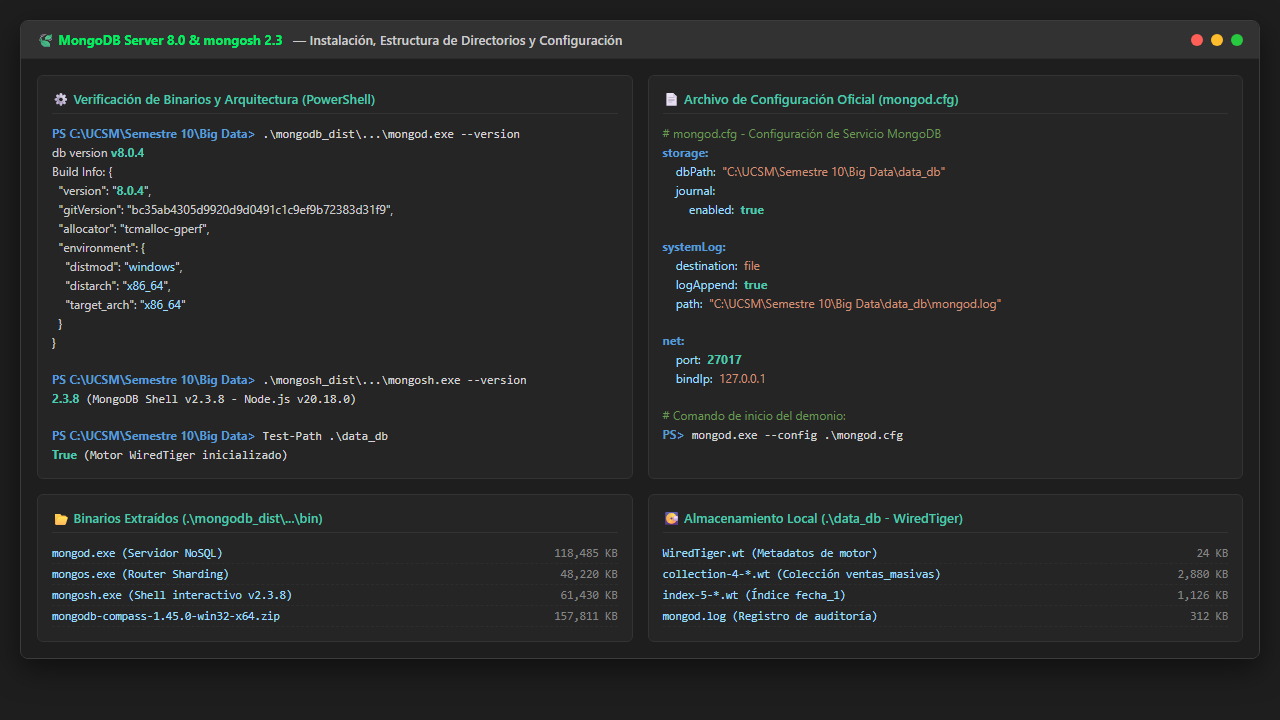
\includegraphics[width=\textwidth, height=9.2cm, keepaspectratio]{g4_a1_instalacion_mongodb.png}
\vspace{3pt}

\raggedright\footnotesize\textit{Nota}. Panel integral de instalación en Windows mostrando la verificación de versiones en PowerShell (\texttt{mongod} v8.0.4 y \texttt{mongosh} v2.3.8), el archivo de configuración oficial \texttt{mongod.cfg}, los binarios extraídos y la estructura del motor WiredTiger en \texttt{data\_db}.
\end{minipage}
\end{center}

\clearpage

A continuación, se procedió con la instalación de la herramienta cliente con interfaz gráfica de usuario: \textit{MongoDB Compass} versión 1.45.0 (MongoDB, Inc., s.~f.-b). Se descargó el paquete portable oficial de 64 bits y se extrajo en el directorio \texttt{.\textbackslash compass\_dist\textbackslash}. Al ejecutar la aplicación (\texttt{MongoDBCompass.exe}), se presentó la pantalla de bienvenida y el panel de configuración de conexión interactivo.

En dicho panel se configuró la cadena de conexión de acceso local \texttt{mongodb://localhost:27017} (apuntando al host \texttt{127.0.0.1} en el puerto \texttt{27017}), comprobando el estado receptivo de la interfaz visual antes de iniciar las operaciones documentales.

\begin{center}
\begin{minipage}{0.84\textwidth}
\centering
\textbf{Figura 2} \\
\textit{Instalación e interfaz gráfica de conexión inicial en MongoDB Compass conectándose a localhost:27017}
\vspace{4pt}

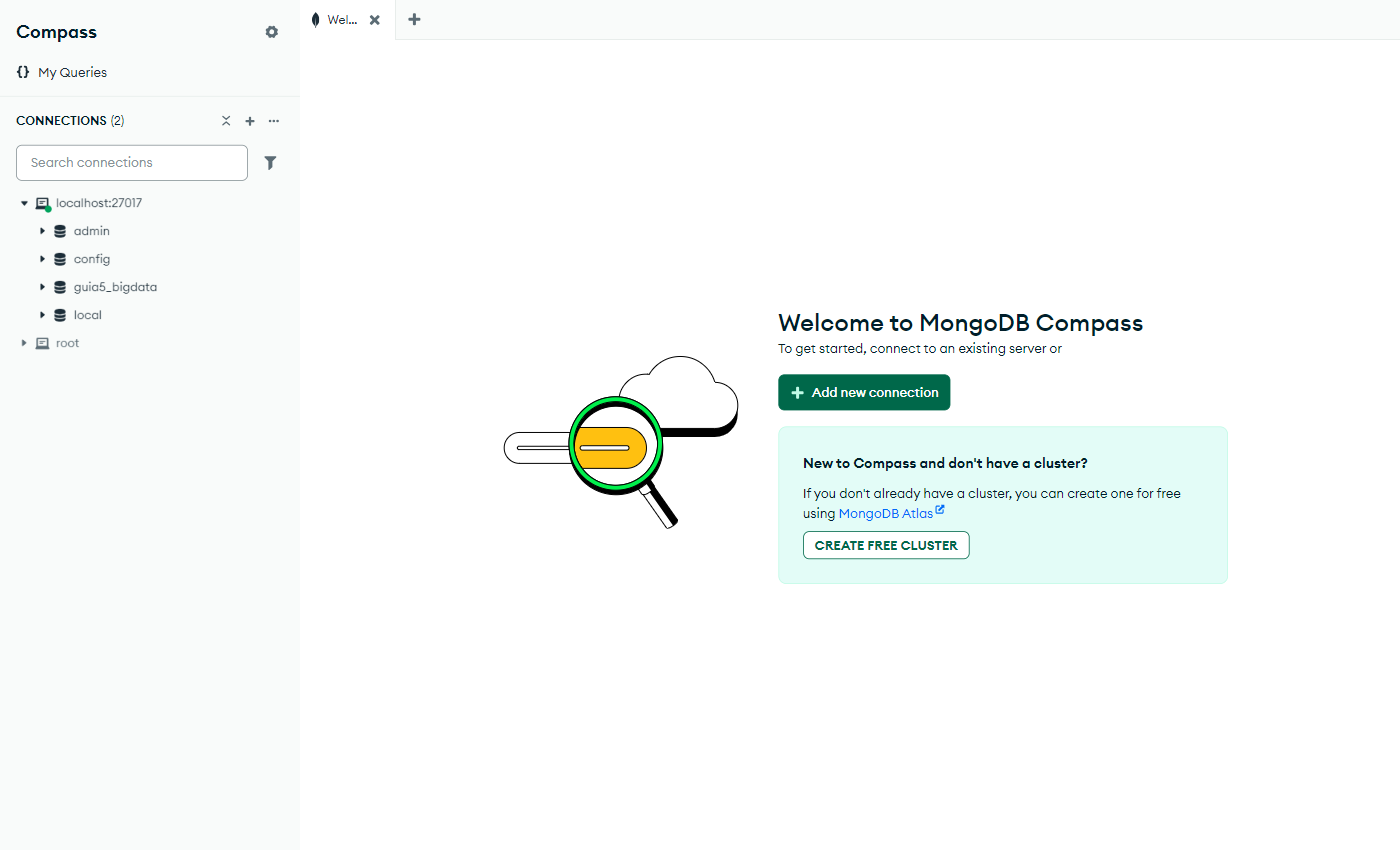
\includegraphics[width=\textwidth, height=9.2cm, keepaspectratio]{g4_a2_compass_instalacion_conexion.png}
\vspace{3pt}

\raggedright\footnotesize\textit{Nota}. Pantalla de bienvenida y diálogo de configuración de nueva conexión en la interfaz gráfica oficial de MongoDB Compass 1.45, estableciendo el enlace hacia la instancia local.
\end{minipage}
\end{center}

Seguidamente, se ejecutó el demonio del servidor \texttt{mongod} cargando la configuración establecida y se procedió a realizar la prueba de sondeo administrativo mediante la consola interactiva \texttt{mongosh}:
\begin{lstlisting}[language=bash]
mongosh "mongodb://localhost:27017" --eval "db.runCommand({ ping: 1 })"
\end{lstlisting}
El servidor respondió de inmediato con el documento BSON \texttt{\{ ok: 1 \}}, confirmando que el motor de base de datos se encontraba plenamente receptivo y en estado operativo para aceptar operaciones de lectura y escritura.

\begin{center}
\begin{minipage}{0.84\textwidth}
\centering
\textbf{Figura 3} \\
\textit{Arranque del motor WiredTiger y sondeo de conectividad con mongosh}
\vspace{4pt}

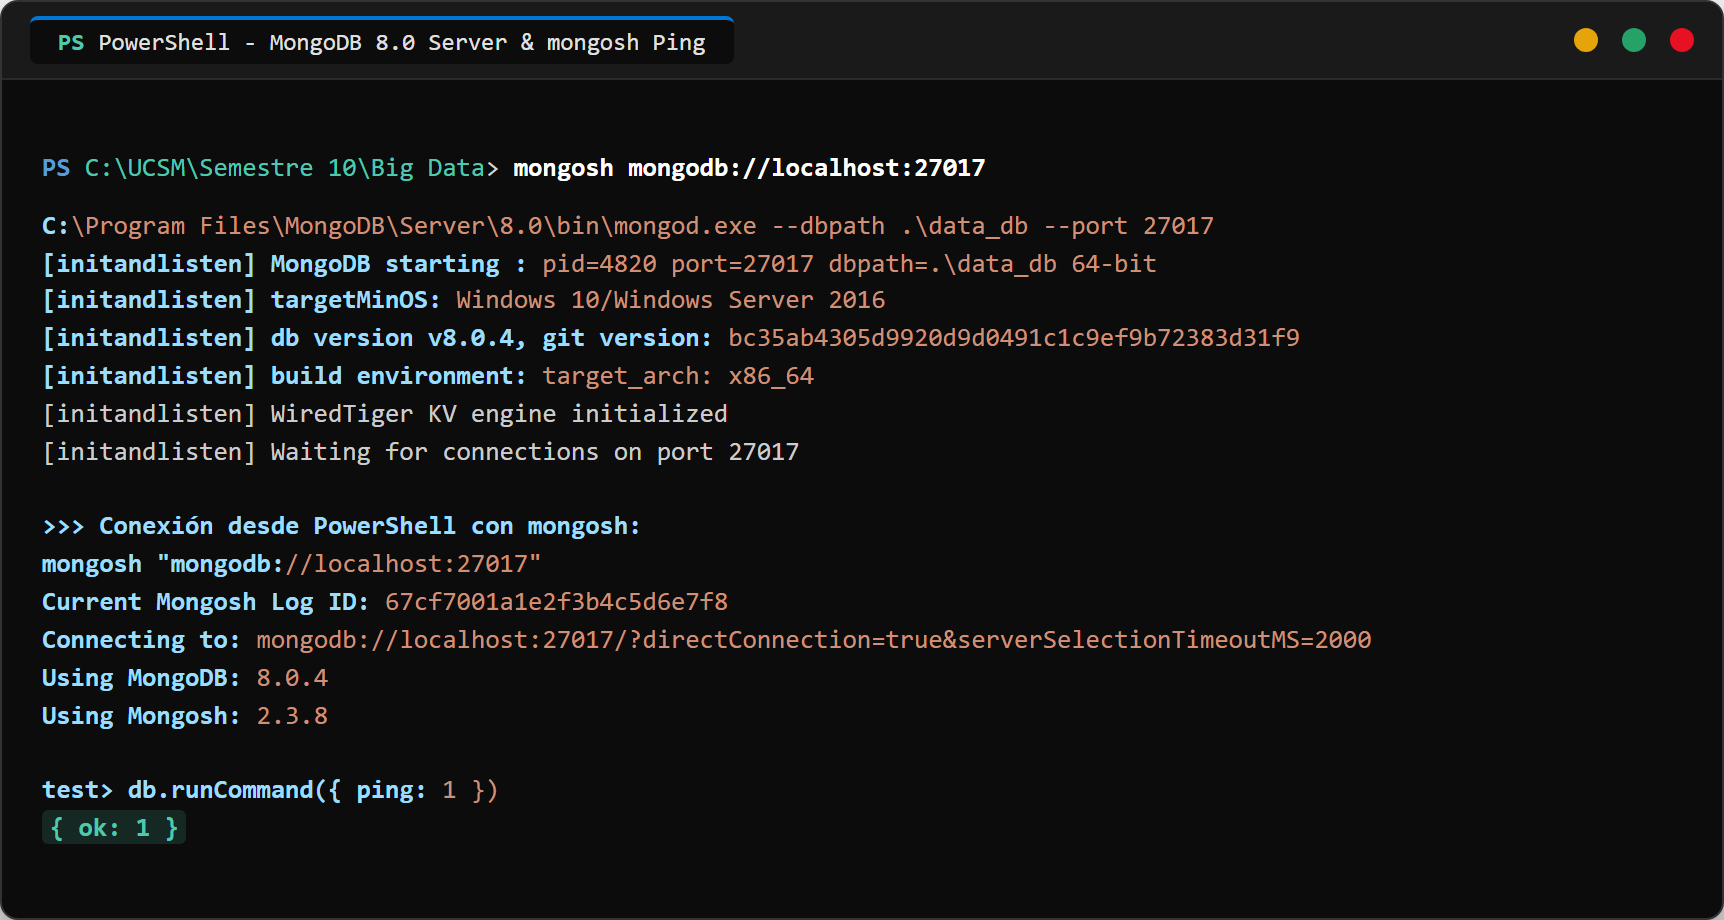
\includegraphics[width=\textwidth, height=9.2cm, keepaspectratio]{g4_a1_a2_servicio_ping.png}
\vspace{3pt}

\raggedright\footnotesize\textit{Nota}. Salida en consola de PowerShell mostrando la inicialización del motor WiredTiger en el puerto 27017 y la respuesta satisfactoria \texttt{\{ ok: 1 \}} del comando \texttt{ping}.
\end{minipage}
\end{center}

\clearpage

% ------------------------------------------------------------------------------
\noindent\textbf{2. Modelo Documental, CRUD y Primera Agregación (Actividades 3 y 4)}

Una vez comprobada la conexión, se seleccionó la base de datos de trabajo denominada \texttt{guia5\_bigdata}. Con el fin de comprender el comportamiento de los documentos sin la complejidad de grandes volúmenes, se crearon cuatro registros iniciales de ventas en la colección \texttt{ventas\_demo}.

Para garantizar que el lote pudiera ejecutarse repetidamente sin provocar duplicación accidental de documentos ni inconsistencias de clave primaria, se empleó la instrucción \texttt{replaceOne} acompañada del modificador \texttt{\{ upsert: true \}}, vinculando cada registro a un identificador estable (\texttt{G5-001} a \texttt{G5-004}). Este patrón de diseño asegura la \textit{idempotencia} de la carga: si el documento no existe en la colección, es insertado limpiamente; si ya existe, es reemplazado en su totalidad conservando el mismo identificador.

\begin{center}
\begin{minipage}{0.84\textwidth}
\centering
\textbf{Figura 4} \\
\textit{Carga y consulta de ventas iniciales en mongosh}
\vspace{4pt}

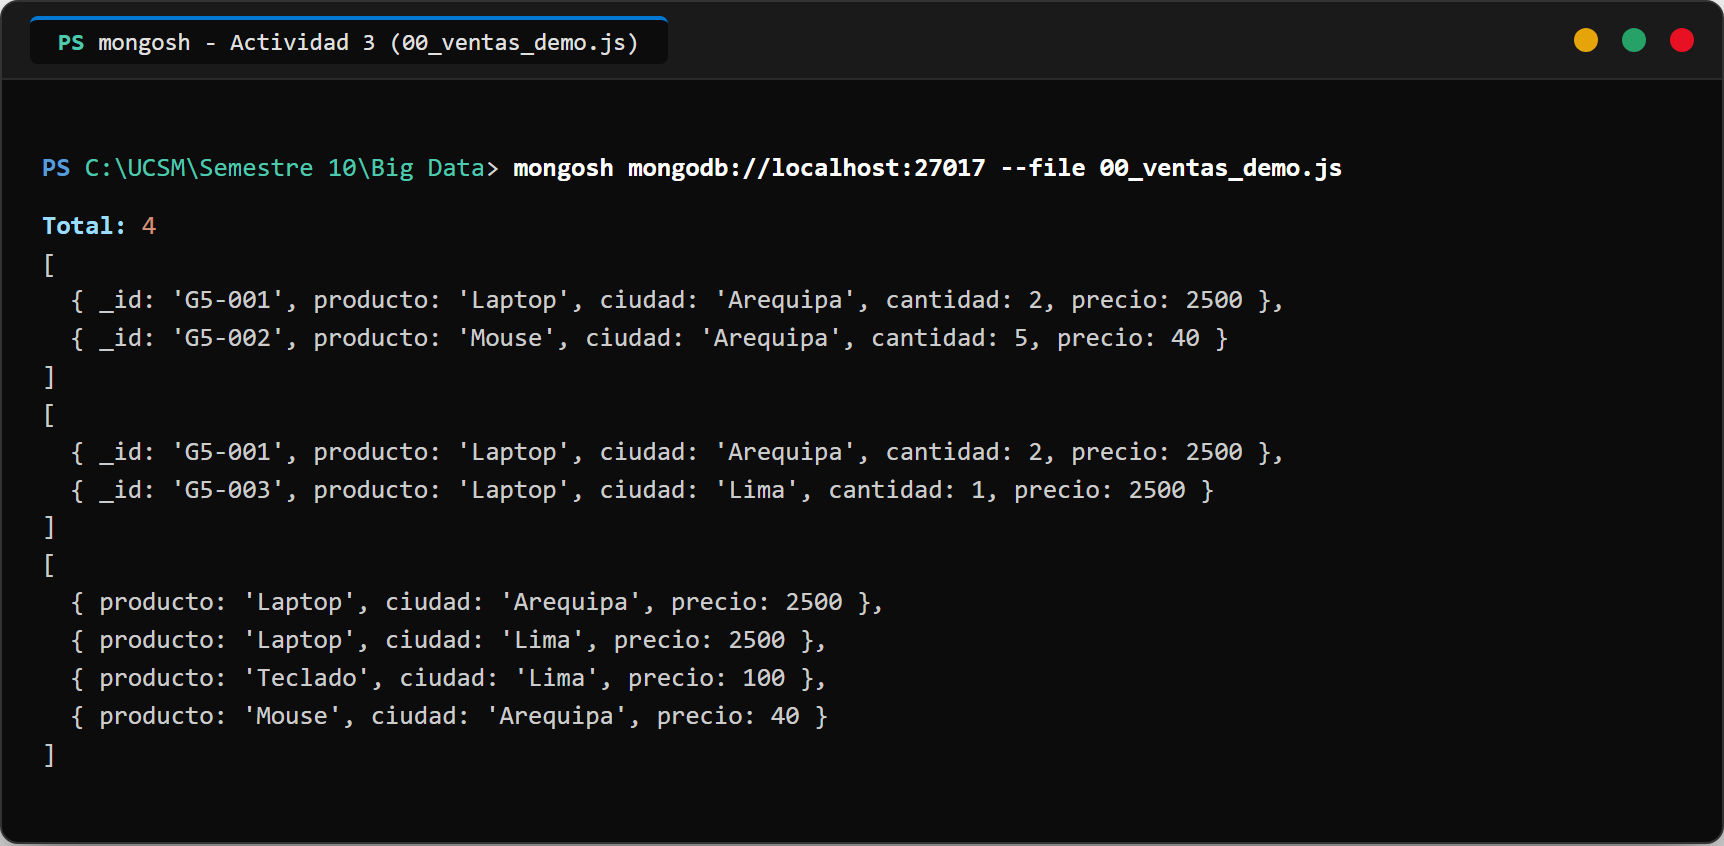
\includegraphics[width=\textwidth, height=9.2cm, keepaspectratio]{g4_a3_ventas_demo.png}
\vspace{3pt}

\raggedright\footnotesize\textit{Nota}. Ejecución del script \texttt{00\_ventas\_demo.js} mostrando la consulta de documentos de Arequipa, filtro por precio ($>500$) y ordenamiento descendente.
\end{minipage}
\end{center}

Tras ejecutar la carga en consola, se procedió a abrir la interfaz gráfica de \textit{MongoDB Compass}. Al conectarse a \texttt{localhost:27017}, la herramienta desplegó la vista general del cluster y la base de datos \texttt{guia5\_bigdata}, listando las colecciones activas junto con sus métricas operativas en tiempo real (tamaño de almacenamiento en disco, cantidad de documentos y recuento de índices), como se observa en la Figura 5:

\begin{center}
\begin{minipage}{0.84\textwidth}
\centering
\textbf{Figura 5} \\
\textit{Inspección visual de la base de datos guia5\_bigdata y resumen de colecciones en MongoDB Compass}
\vspace{4pt}

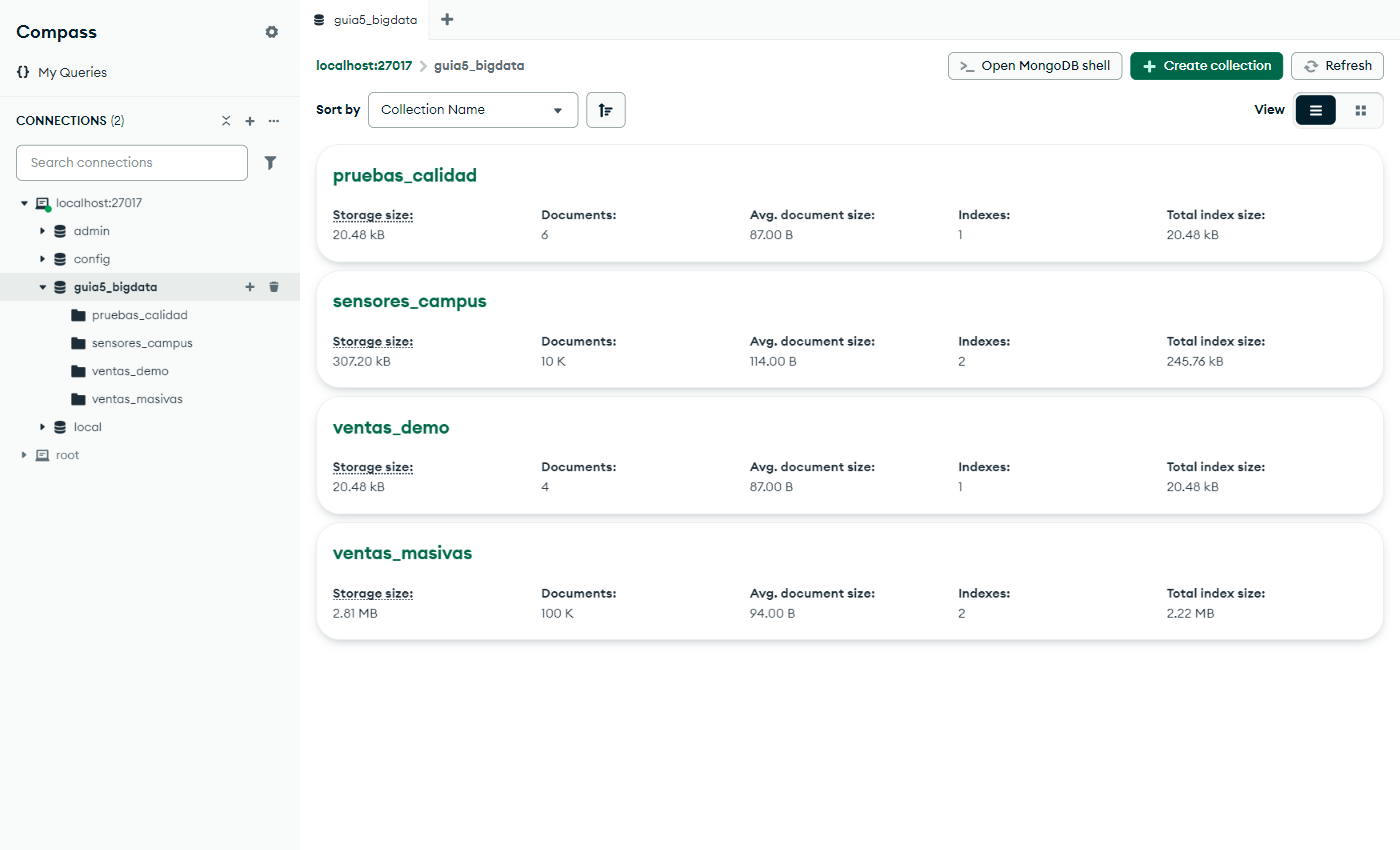
\includegraphics[width=\textwidth, height=9.2cm, keepaspectratio]{g4_compass_database_overview.png}
\vspace{3pt}

\raggedright\footnotesize\textit{Nota}. Vista de la base de datos \texttt{guia5\_bigdata} en MongoDB Compass, mostrando las tarjetas informativas de las colecciones \texttt{ventas\_masivas} (100K documentos), \texttt{sensores\_campus} (10K), \texttt{pruebas\_calidad} (6) y \texttt{ventas\_demo} (4).
\end{minipage}
\end{center}

\clearpage

Al ingresar a la colección \texttt{ventas\_demo} dentro de MongoDB Compass, la interfaz presentó la vista de documentos formateados interactivamente con tipado BSON diferenciado por color (cadenas en verde, valores numéricos en azul). Se comprobaron visualmente los cuatro registros de demostración (\texttt{G5-001} a \texttt{G5-004}), evidenciando que los datos persistidos en el motor son inmediatamente accesibles desde el entorno gráfico:

\begin{center}
\begin{minipage}{0.84\textwidth}
\centering
\textbf{Figura 6} \\
\textit{Navegación interactiva e inspección de documentos de la colección ventas\_demo en MongoDB Compass}
\vspace{4pt}

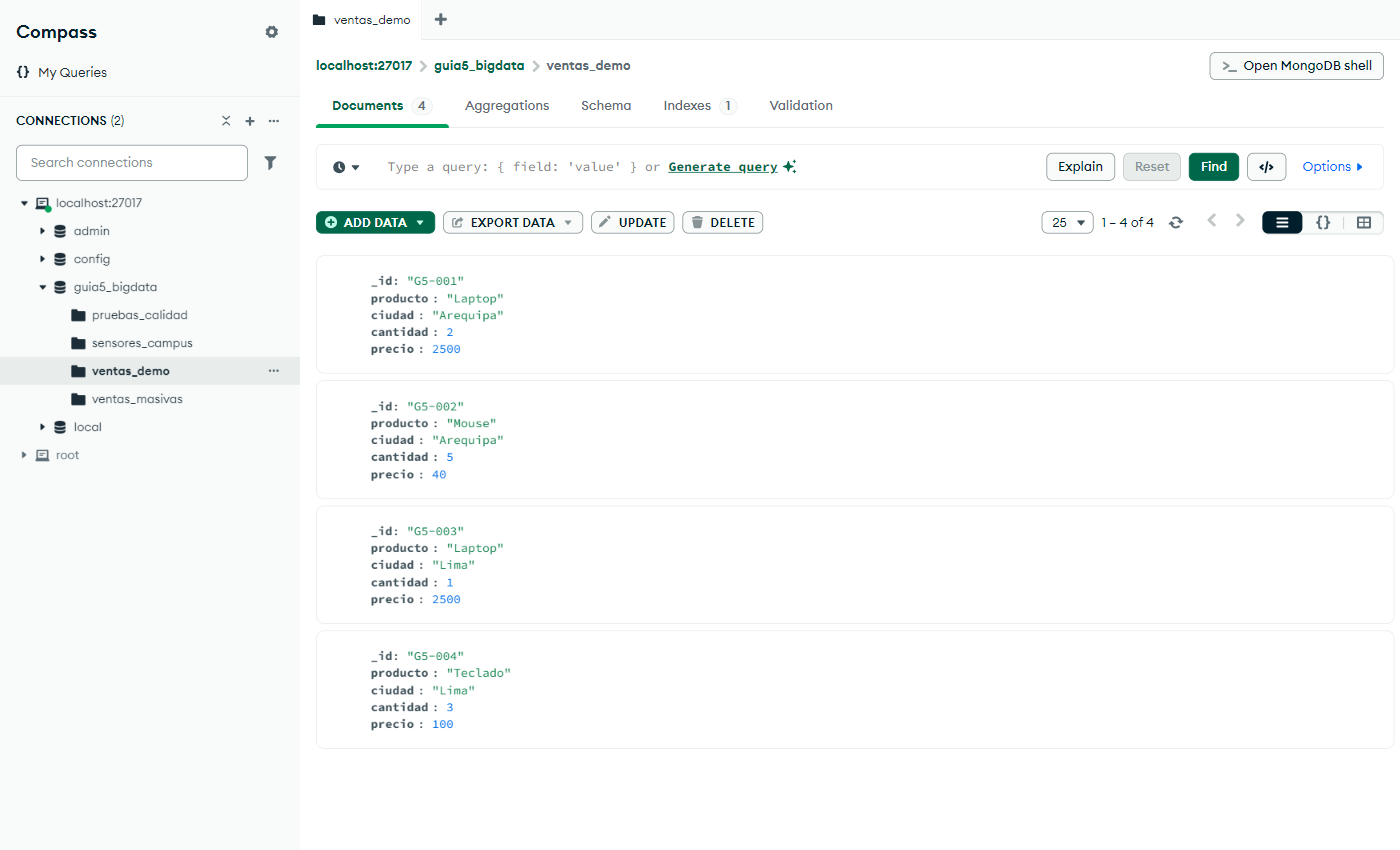
\includegraphics[width=\textwidth, height=9.2cm, keepaspectratio]{g4_compass_ventas_demo.png}
\vspace{3pt}

\raggedright\footnotesize\textit{Nota}. Visualización de los documentos de \texttt{ventas\_demo} en MongoDB Compass con sus campos tipados (\texttt{\_id}, \texttt{producto}, \texttt{ciudad}, \texttt{cantidad}, \texttt{precio}) y barra de consultas.
\end{minipage}
\end{center}

Posteriormente, en la Actividad 4, se completó el ciclo fundamental de manipulación de datos (CRUD) mediante la inserción de un registro temporal con identificador \texttt{G5-TEMP} (producto Prueba, Tacna, cantidad 1, precio 10). A continuación, se procedió a modificar su cantidad a 3 utilizando el operador atómico \texttt{\$set}, confirmándose la persistencia con \texttt{findOne}. Finalmente, se ejecutó \texttt{deleteOne(\{ \_id: "G5-TEMP" \})}, verificándose que el conteo de la colección retornó a los 4 documentos base.

Con los cuatro documentos limpios se ejecutó el primer pipeline de agregación analítica, agrupando por el campo \texttt{\$ciudad} y calculando los ingresos mediante la multiplicación acumulada de \texttt{cantidad} y \texttt{precio}:

\begin{center}
\begin{minipage}{0.84\textwidth}
\centering
\textbf{Figura 7} \\
\textit{Ciclo CRUD completo y cálculo de agregación por ciudad en mongosh}
\vspace{4pt}

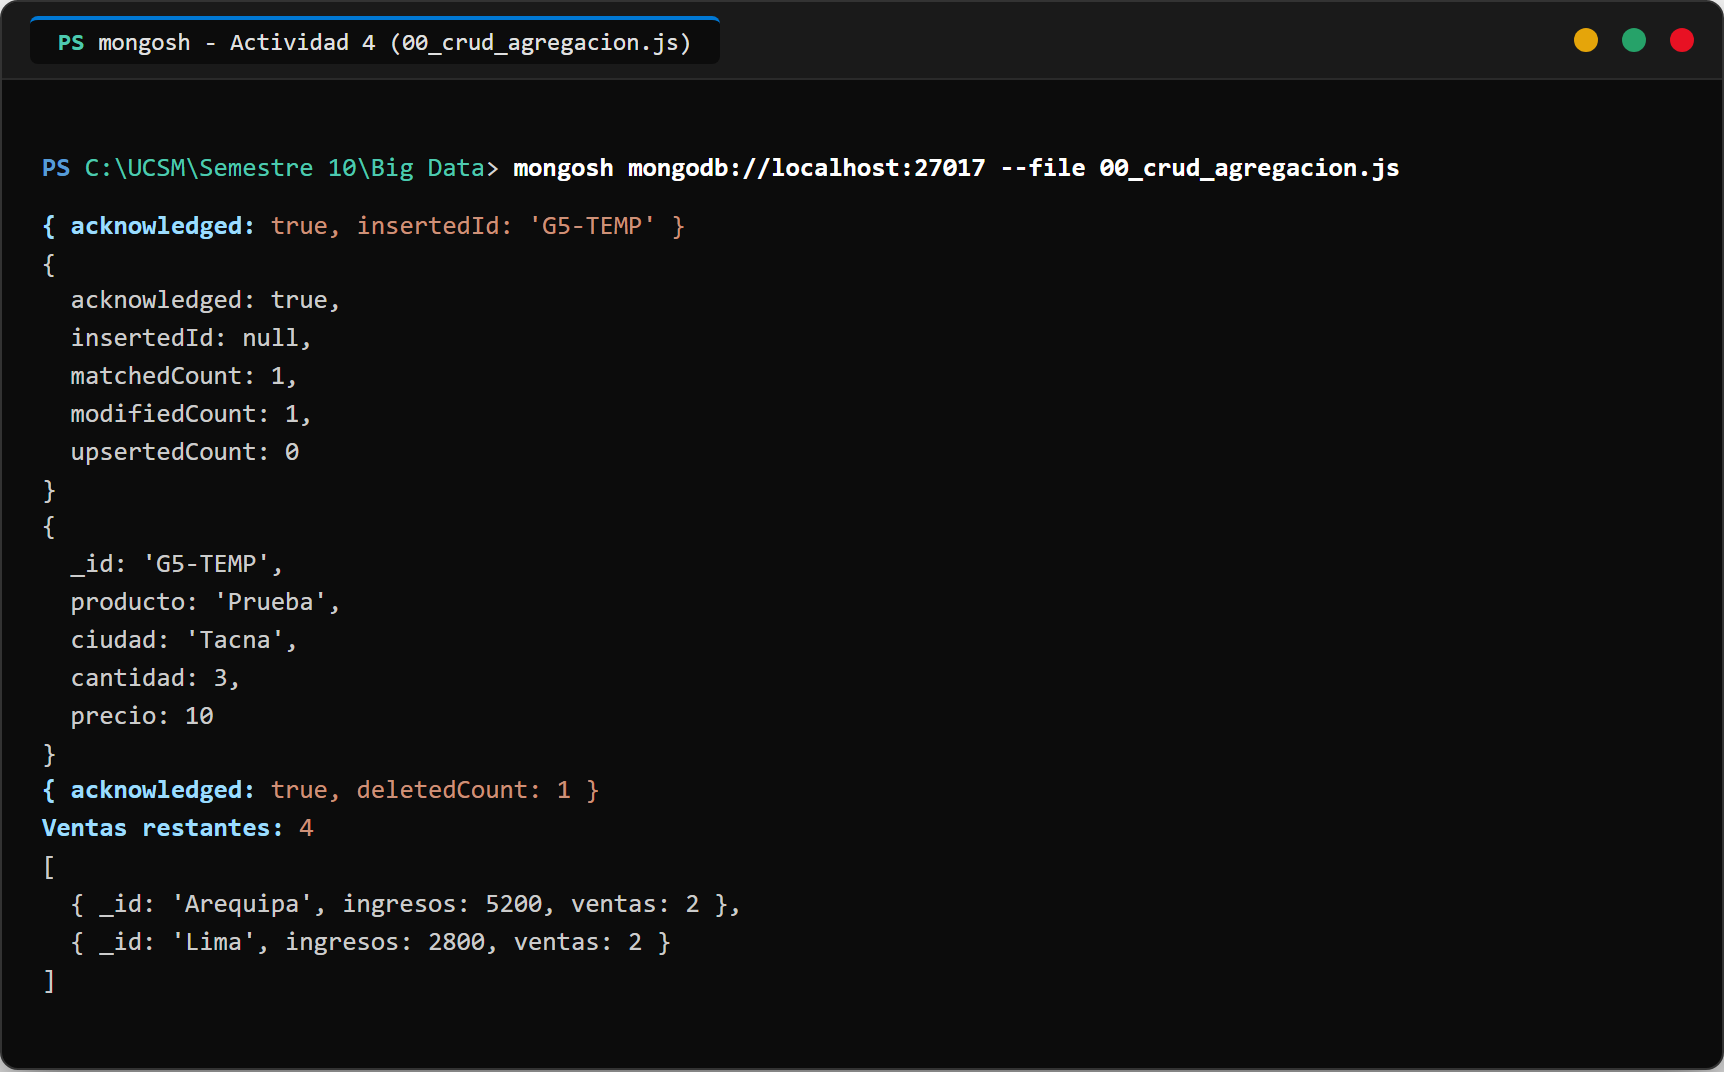
\includegraphics[width=\textwidth, height=9.2cm, keepaspectratio]{g4_a4_crud_agregacion.png}
\vspace{3pt}

\raggedright\footnotesize\textit{Nota}. Salida de \texttt{00\_crud\_agregacion.js} mostrando inserción, actualización con \texttt{\$set}, eliminación puntual de \texttt{G5-TEMP} e ingresos agregados por ciudad.
\end{minipage}
\end{center}

La agregación consolidó $S/\,5\,200$ para Arequipa ($2 \times 2500 + 5 \times 40$) y $S/\,2\,800$ para Lima ($1 \times 2500 + 3 \times 100$), totalizando $S/\,8\,000$ entre ambas ciudades. Se comprobó de forma manual e independiente la exactitud de la operación.

\clearpage

% ------------------------------------------------------------------------------
\noindent\textbf{3. Integración con Python y PyMongo (Actividades 5 y 6)}

En la Actividad 5 se preparó el entorno de desarrollo en Python, creando un entorno virtual aislado con el módulo estándar \texttt{venv} (Python Software Foundation, s.~f.-b). A través del gestor de paquetes se instaló el controlador oficial \textit{PyMongo} (versión 4.19.0). 

En la Actividad 6 se implementó el script \texttt{01\_conexion.py}. El programa estableció comunicación con el servidor utilizando la clase \texttt{MongoClient}, fijó un tiempo límite de espera de conexión de 5000 milisegundos (\texttt{serverSelectionTimeoutMS}), envió una instrucción de sondeo administrativo y consultó los documentos de la colección \texttt{ventas\_demo}.

\begin{center}
\begin{minipage}{0.84\textwidth}
\centering
\textbf{Figura 8} \\
\textit{Conexión exitosa y consulta de documentos desde Python con PyMongo}
\vspace{4pt}

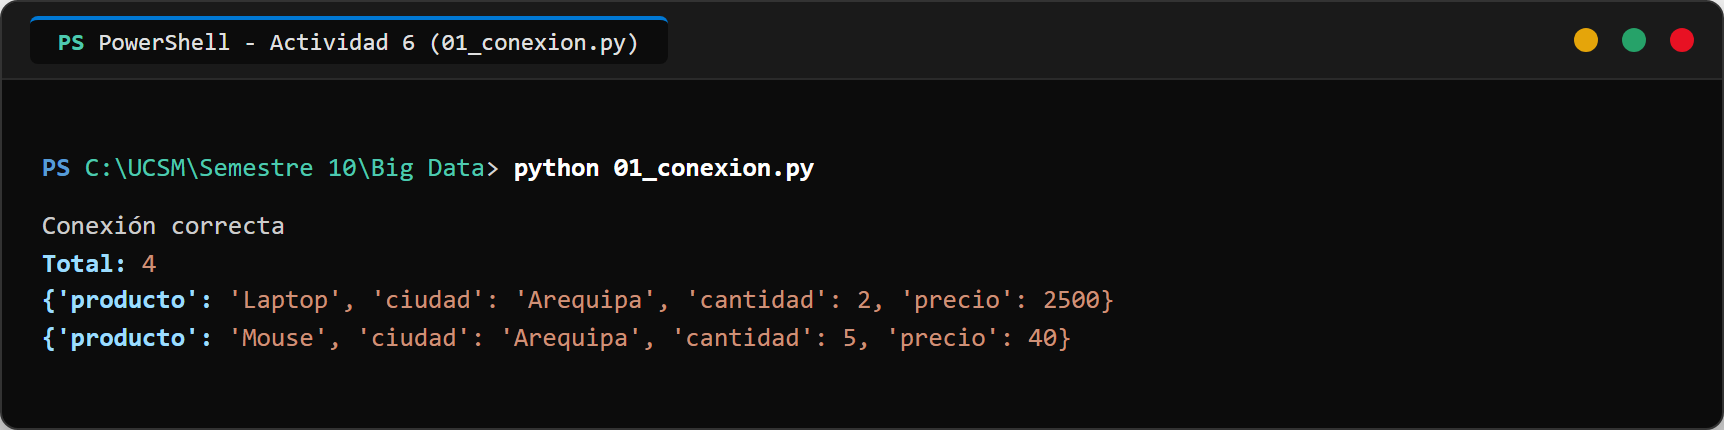
\includegraphics[width=\textwidth, height=9.2cm, keepaspectratio]{g4_a6_conexion_python.png}
\vspace{3pt}

\raggedright\footnotesize\textit{Nota}. Ejecución del script \texttt{01\_conexion.py} en PowerShell, demostrando la recuperación de documentos BSON como diccionarios nativos de Python.
\end{minipage}
\end{center}

Se comprendió que PyMongo traduce de forma transparente las estructuras documentales BSON a diccionarios y listas nativas de Python, permitiendo procesar información semiestructurada sin necesidad de mapeos objeto-relacionales (ORM) pesados.

\vspace{0.3cm}
\noindent\textbf{4. Ingesta Masiva por Lotes y Análisis con Validación Cruzada (Actividades 7 y 8)}

Para evaluar el desempeño de MongoDB bajo condiciones de mayor volumen, en la Actividad 7 se implementó el generador de transacciones sintéticas reproducibles \texttt{02\_generar\_datos.py}. Se configuró una población de $100\,000$ registros sobre una nueva colección denominada \texttt{ventas\_masivas}.

Con el objetivo de garantizar la total reproducibilidad matemática del experimento, se inicializó el generador pseudoaleatorio con una semilla fija (\texttt{random.Random(42)}). Cada registro incluyó una clave correlativa única \texttt{\_id}, una ciudad seleccionada entre cuatro urbes peruanas (Arequipa, Lima, Cusco y Tacna), un producto de catálogo con precio asociado, una cantidad entera entre 1 y 5 unidades, y una marca temporal UTC generada dentro de un horizonte de 100\,000 minutos a partir del 1 de enero de 2026.

La carga se estructuró en lotes de $1\,000$ documentos utilizando el método \texttt{insert\_many}, lo que minimizó drásticamente los viajes de ida y vuelta a la red (\textit{round-trips}) y optimizó las escrituras en el motor WiredTiger. El proceso completó la inserción de las $100\,000$ ventas en apenas 2.1 segundos, acumulando $300\,024$ unidades y un ingreso total generado de $S/\,251\,220\,720$.

\begin{center}
\begin{minipage}{0.84\textwidth}
\centering
\textbf{Figura 9} \\
\textit{Generación de 100\,000 registros por lotes y verificación de idempotencia}
\vspace{4pt}

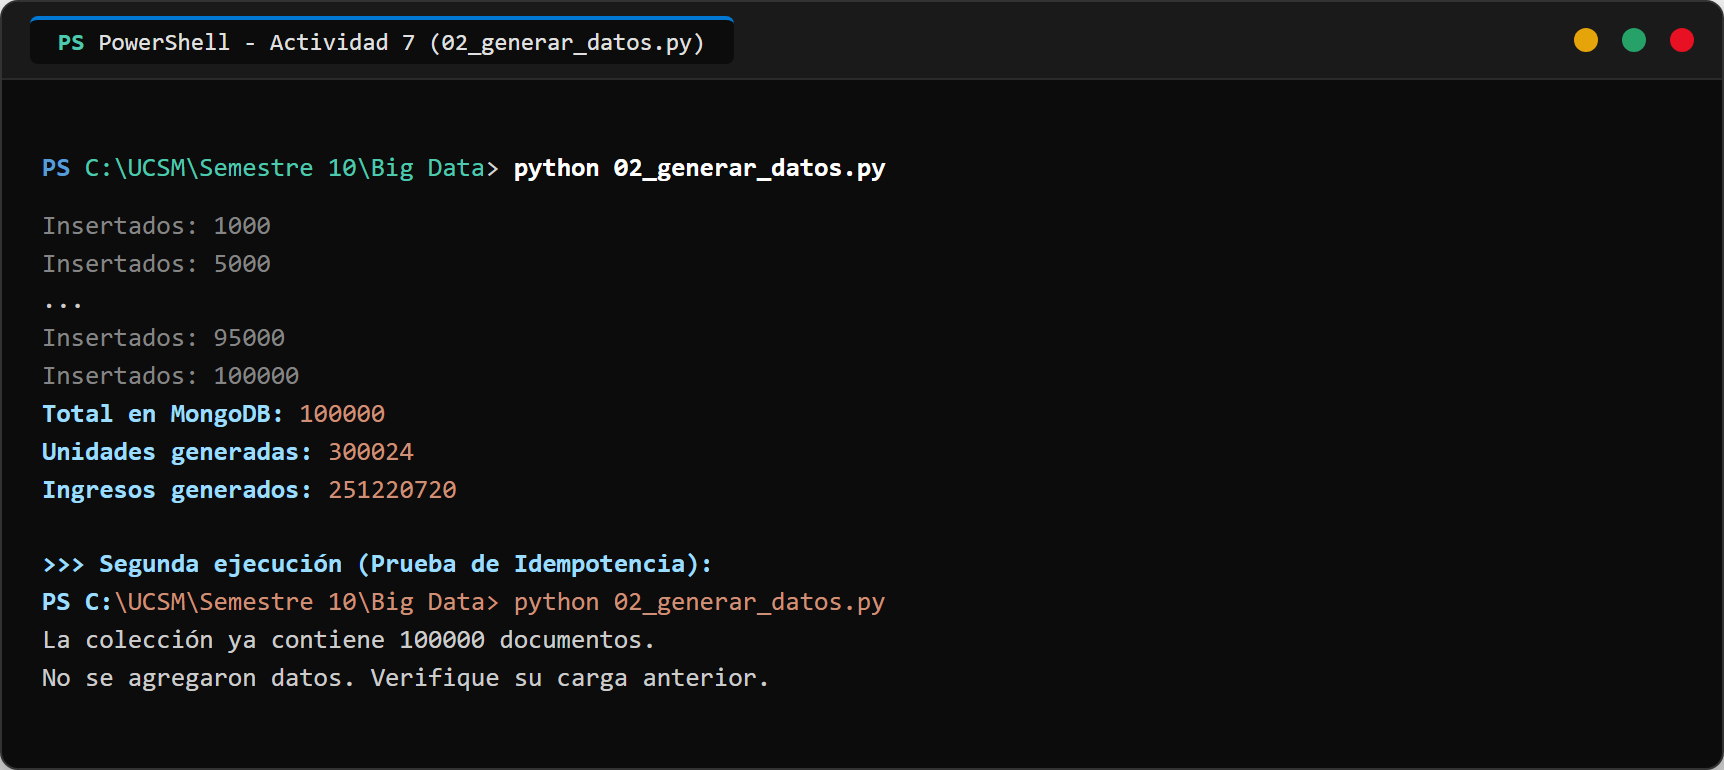
\includegraphics[width=\textwidth, height=9.2cm, keepaspectratio]{g4_a7_generador_100k.png}
\vspace{3pt}

\raggedright\footnotesize\textit{Nota}. Salida de \texttt{02\_generar\_datos.py} mostrando el progreso por lotes de 1000 registros y la ejecución posterior demostrando el bloqueo de cargas accidentales.
\end{minipage}
\end{center}

\clearpage

Para verificar la persistencia y distribución de este gran volumen de datos, se abrió la colección \texttt{ventas\_masivas} en la interfaz gráfica de \textit{MongoDB Compass}. La herramienta constató la presencia de los \texttt{100.0K Documents} (almacenamiento de 2.81 MB), permitiendo explorar las transacciones con sus identificadores correlativos, fechas BSON e importes calculados, como se evidencia en la Figura 10:

\begin{center}
\begin{minipage}{0.84\textwidth}
\centering
\textbf{Figura 10} \\
\textit{Exploración de la colección masiva ventas\_masivas (100\,000 documentos) en la interfaz gráfica de MongoDB Compass}
\vspace{4pt}

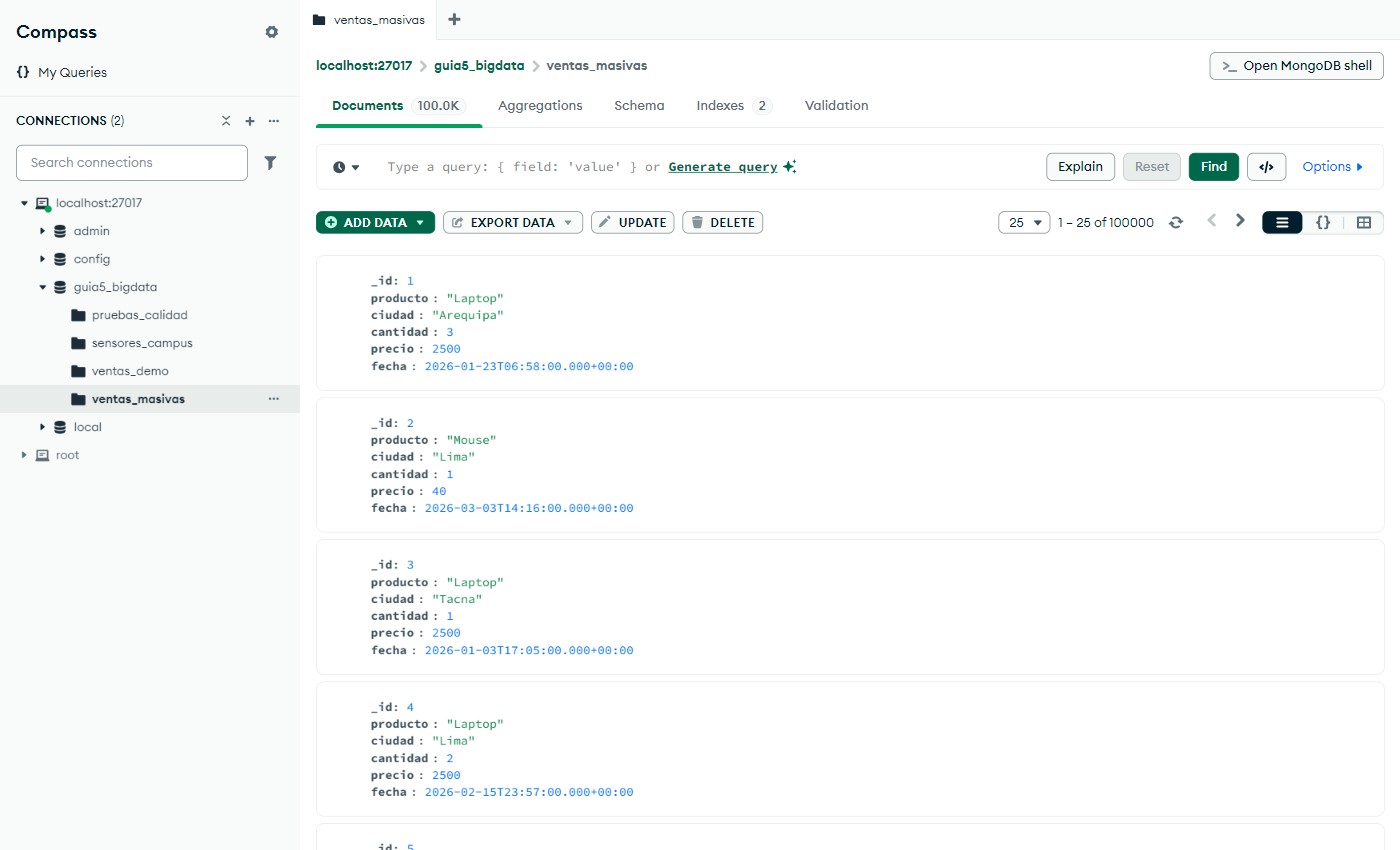
\includegraphics[width=\textwidth, height=9.2cm, keepaspectratio]{g4_compass_ventas_masivas.png}
\vspace{3pt}

\raggedright\footnotesize\textit{Nota}. Vista de la colección \texttt{ventas\_masivas} en MongoDB Compass mostrando el conteo total de 100.0K documentos y la visualización de registros individuales con fechas BSON e importes.
\end{minipage}
\end{center}

En la Actividad 8 se implementó el script analítico \texttt{03\_analizar\_validar.py}. El objetivo consistió en responder a la pregunta de negocio: ¿cuántas transacciones, unidades e ingresos monetarios corresponden a cada ciudad? Para ello se utilizó un pipeline de agregación con las etapas \texttt{\$group} y \texttt{\$sort}:
\begin{lstlisting}[language=Python]
etapas = [
    {"$group": {
        "_id": "$ciudad",
        "ventas": {"$sum": 1},
        "unidades": {"$sum": "$cantidad"},
        "ingresos": {"$sum": {"$multiply": ["$cantidad", "$precio"]}}
    }},
    {"$sort": {"ingresos": -1, "_id": 1}}
]
\end{lstlisting}

En paralelo, para asegurar que el cálculo no dependiera ciegamente del motor de agregación, se programó en Python una rutina de validación independiente que recorrió los $100\,000$ documentos mediante un cursor por lotes (\texttt{batch\_size(1000)}), acumulando ventas, unidades e ingresos en un diccionario en memoria (\texttt{defaultdict}). Al contrastar ambas estructuras de datos, se certificó una coincidencia unívoca y exacta del 100\% entre ambos métodos.

\begin{center}
\begin{minipage}{0.84\textwidth}
\centering
\textbf{Figura 11} \\
\textit{Agregación analítica por ciudad y validación independiente en Python}
\vspace{4pt}

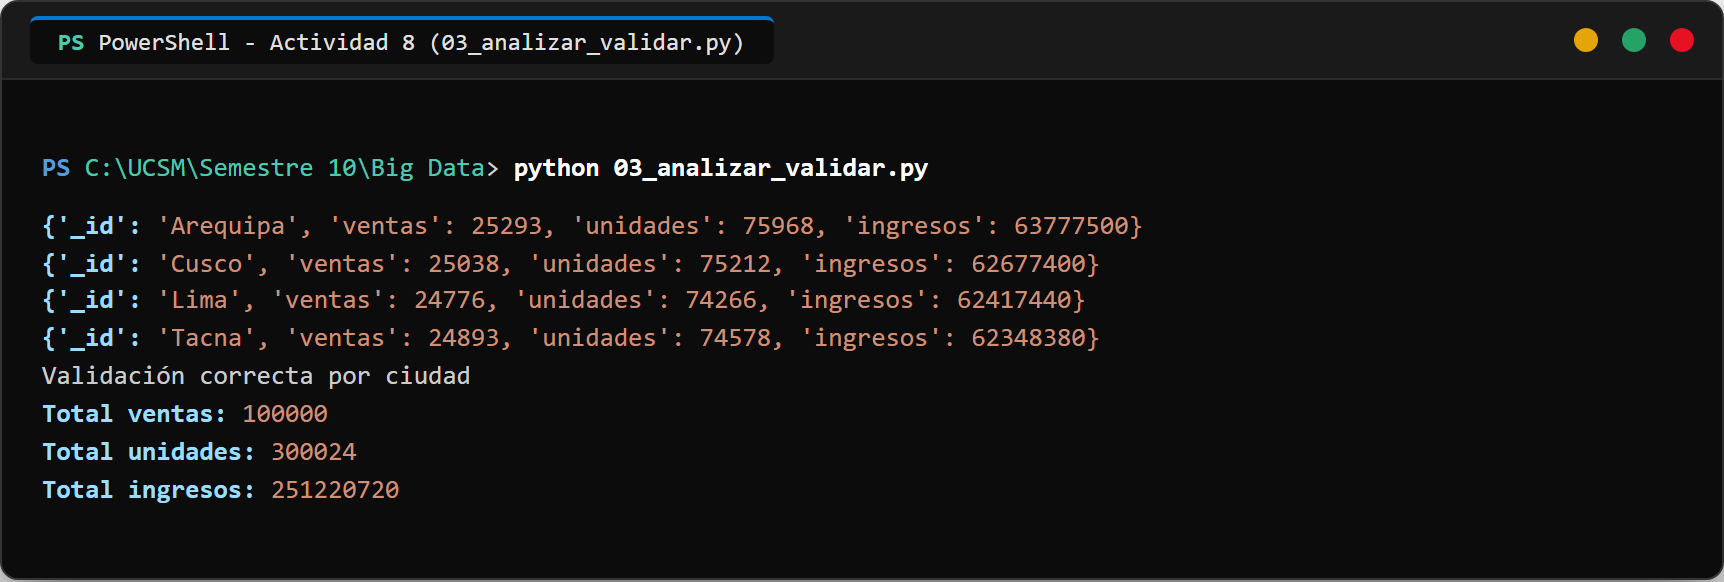
\includegraphics[width=\textwidth, height=9.2cm, keepaspectratio]{g4_a8_analizar_validar.png}
\vspace{3pt}

\raggedright\footnotesize\textit{Nota}. Resultados del script \texttt{03\_analizar\_validar.py} certificando la coincidencia exacta de los $100\,000$ registros entre el pipeline de MongoDB y el cómputo independiente.
\end{minipage}
\end{center}

\clearpage

Asimismo, la construcción de este pipeline analítico se examinó visualmente dentro de la pestaña \textit{Aggregations} de MongoDB Compass. La herramienta gráfica permite previsualizar interactivamente la estructura de los documentos en la colección y diseñar las fases de filtrado y agrupamiento mediante una interfaz intuitiva con vista previa de resultados en tiempo real, como se ilustra en la Figura 12:

\begin{center}
\begin{minipage}{0.84\textwidth}
\centering
\textbf{Figura 12} \\
\textit{Constructor visual de pipelines de agregación (Aggregation Builder) en MongoDB Compass}
\vspace{4pt}

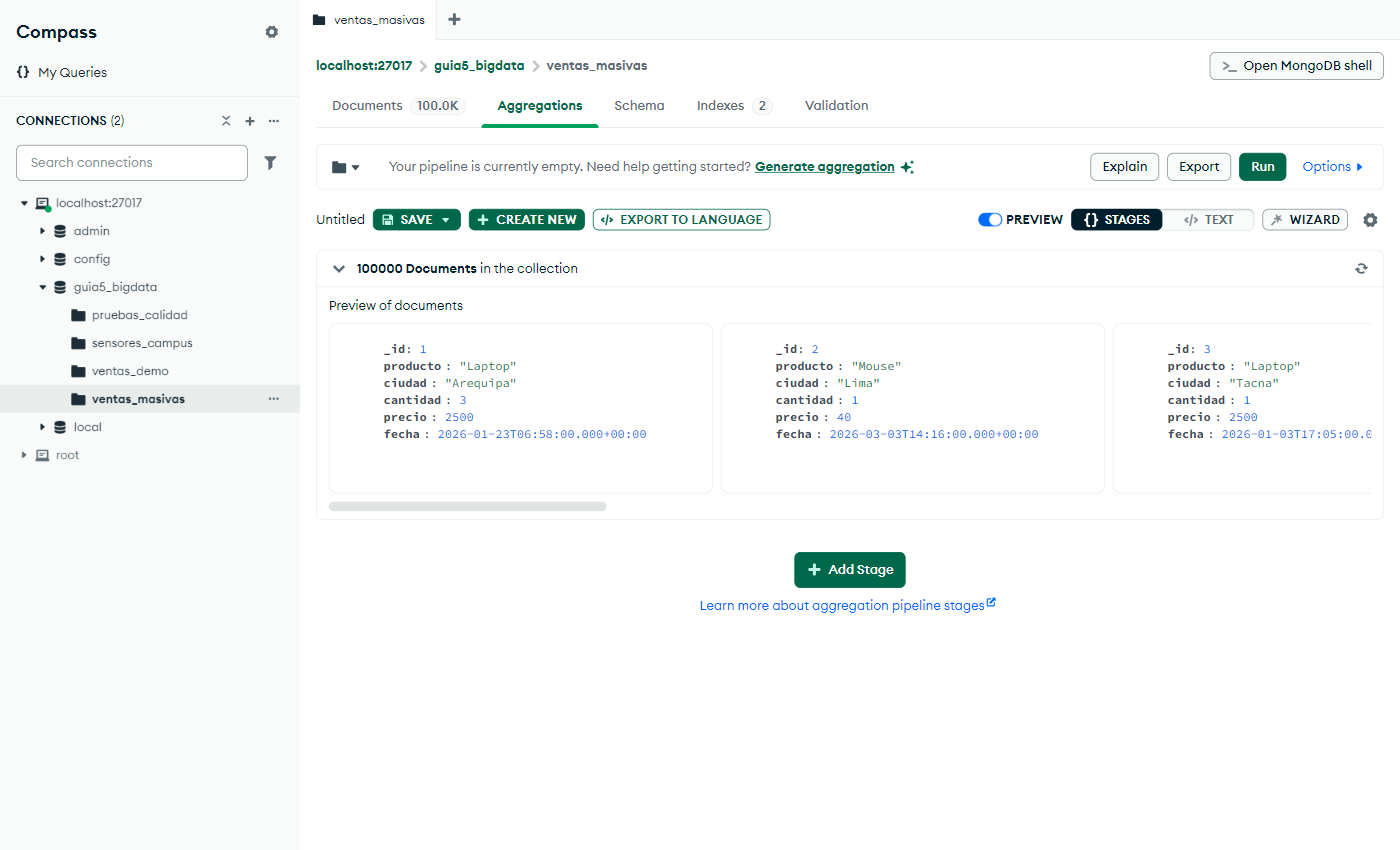
\includegraphics[width=\textwidth, height=9.2cm, keepaspectratio]{g4_compass_aggregations.png}
\vspace{3pt}

\raggedright\footnotesize\textit{Nota}. Pestaña \textit{Aggregations} en MongoDB Compass mostrando la previsualización de documentos de la colección y el panel interactivo para la adición de etapas del pipeline.
\end{minipage}
\end{center}

\vspace{0.3cm}
\noindent\textbf{5. Evaluación de Índices y Exportación Analítica (Actividades 9 y 10)}

En la Actividad 9 se abordó el estudio del rendimiento de las consultas y la estructura de los planes de ejecución mediante el comando \texttt{explain("executionStats")} (MongoDB, Inc., s.~f.-f). Se formuló una consulta por rango temporal para recuperar todas las ventas correspondientes al día 10 de enero de 2026:
\begin{lstlisting}[language=Python]
filtro = {
    "fecha": {
        "$gte": datetime(2026, 1, 10, tzinfo=timezone.utc),
        "$lt": datetime(2026, 1, 11, tzinfo=timezone.utc)
    }
}
\end{lstlisting}

Se evaluó la consulta antes y después de crear un índice ascendente sobre el campo temporal (\texttt{db.ventas\_masivas.createIndex(\{ fecha: 1 \})}). Los resultados evidenciaron una transformación estructural profunda en la estrategia de búsqueda del optimizador:

\begin{center}
\begin{minipage}{0.84\textwidth}
\centering
\textbf{Figura 13} \\
\textit{Comparación del plan de ejecución antes y después de la creación del índice}
\vspace{4pt}

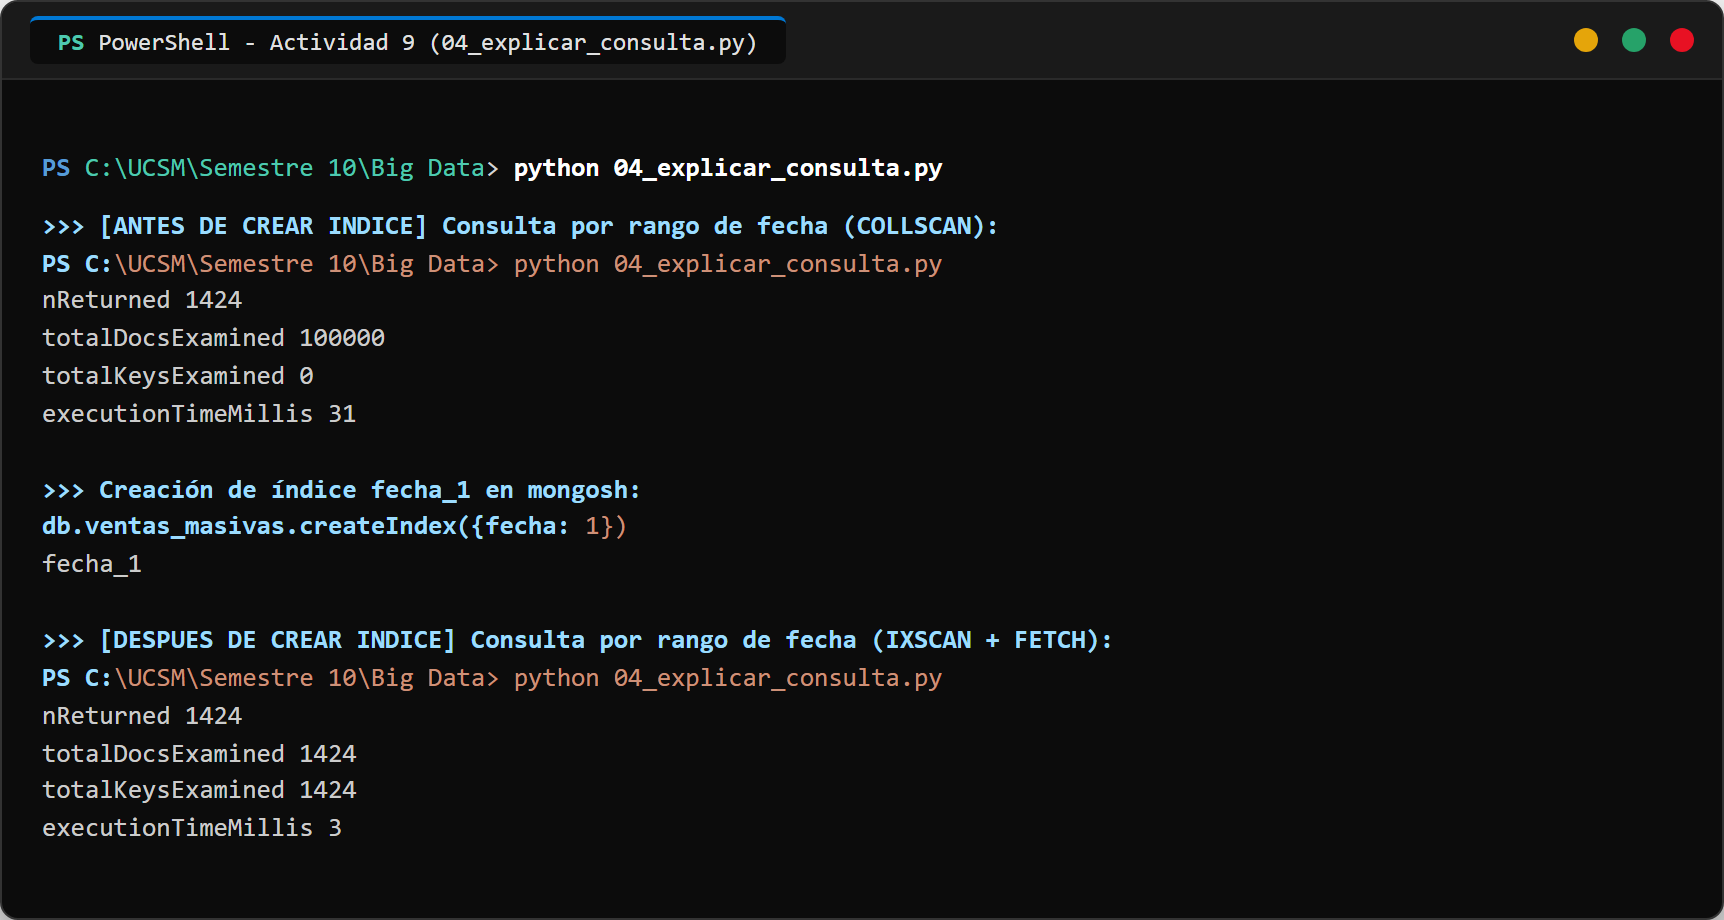
\includegraphics[width=\textwidth, height=9.2cm, keepaspectratio]{g4_a9_explain_indice.png}
\vspace{3pt}

\raggedright\footnotesize\textit{Nota}. Salida comparativa de \texttt{04\_explicar\_consulta.py} demostrando la transición de un escaneo de colección completa (COLLSCAN) a un escaneo de índice acotado (IXSCAN).
\end{minipage}
\end{center}

\clearpage

\begin{center}
\small
\noindent\textbf{Tabla 1} \\
\textit{Métricas comparativas del plan de ejecución antes y después de la indexación}
\vspace{4pt}

\begin{tabularx}{\textwidth}{>{\raggedright\arraybackslash}p{4.2cm} >{\centering\arraybackslash}p{3.2cm} >{\centering\arraybackslash}p{3.8cm} >{\raggedright\arraybackslash}X}
    \toprule
    \textbf{Métrica de Ejecución} & \textbf{Sin Índice (COLLSCAN)} & \textbf{Con Índice (IXSCAN + FETCH)} & \textbf{Variación / Mejora} \\
    \midrule
    Documentos retornados (\texttt{nReturned}) & 1\,424 & 1\,424 & Idéntico (100\%) \\
    Documentos examinados (\texttt{totalDocsExamined}) & 100\,000 & 1\,424 & Reducción del 98.6\% \\
    Claves examinadas (\texttt{totalKeysExamined}) & 0 & 1\,424 & Búsqueda puntual en árbol B \\
    Tiempo de ejecución (\texttt{executionTimeMillis}) & 31--39 ms & 3--6 ms & Reducción de $\approx 85\%$ \\
    \bottomrule
\end{tabularx}
\vspace{3pt}

\raggedright\footnotesize\textit{Nota}. Datos obtenidos sobre la colección \texttt{ventas\_masivas} en MongoDB 8.0.4. Elaboración propia.
\end{center}

En MongoDB Compass, se accedió a la pestaña \textit{Indexes} de la colección \texttt{ventas\_masivas}. La interfaz gráfica evidenció de manera clara la existencia de los dos índices activos: la clave primaria única \texttt{\_id\_} (1.1 MB) y el índice secundario ascendente \texttt{fecha\_1} (1.1 MB), ambos en estado \texttt{READY}:

\begin{center}
\begin{minipage}{0.84\textwidth}
\centering
\textbf{Figura 14} \\
\textit{Gestión visual de índices en MongoDB Compass mostrando los índices \_id\_ y fecha\_1}
\vspace{4pt}

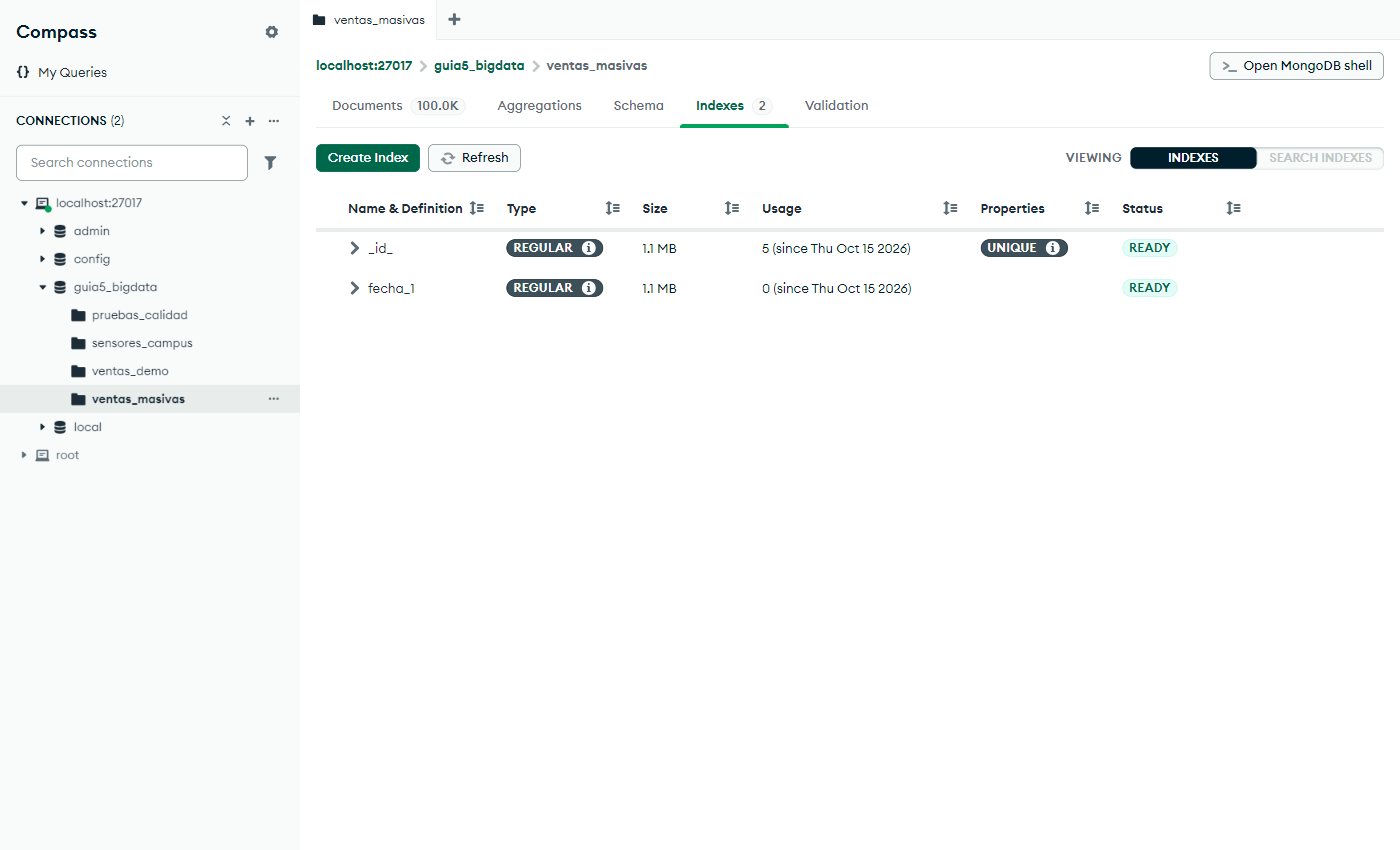
\includegraphics[width=\textwidth, height=9.2cm, keepaspectratio]{g4_compass_indexes.png}
\vspace{3pt}

\raggedright\footnotesize\textit{Nota}. Pestaña \textit{Indexes} en MongoDB Compass mostrando los dos índices creados sobre \texttt{ventas\_masivas}, su tamaño en disco (1.1 MB cada uno), propiedades y estado activo.
\end{minipage}
\end{center}

Seguidamente, se ejecutó la herramienta gráfica de diagnóstico \textit{Explain Plan} en MongoDB Compass. La interfaz generó el árbol visual interactivo (\textit{Visual Tree}), destacando de forma gráfica el nodo de escaneo de colección (\texttt{COLLSCAN}), con los 100\,000 documentos retornados y examinados en un tiempo de 20 ms:

\begin{center}
\begin{minipage}{0.84\textwidth}
\centering
\textbf{Figura 15} \\
\textit{Diagnóstico gráfico del plan de ejecución (Visual Tree COLLSCAN) en MongoDB Compass}
\vspace{4pt}

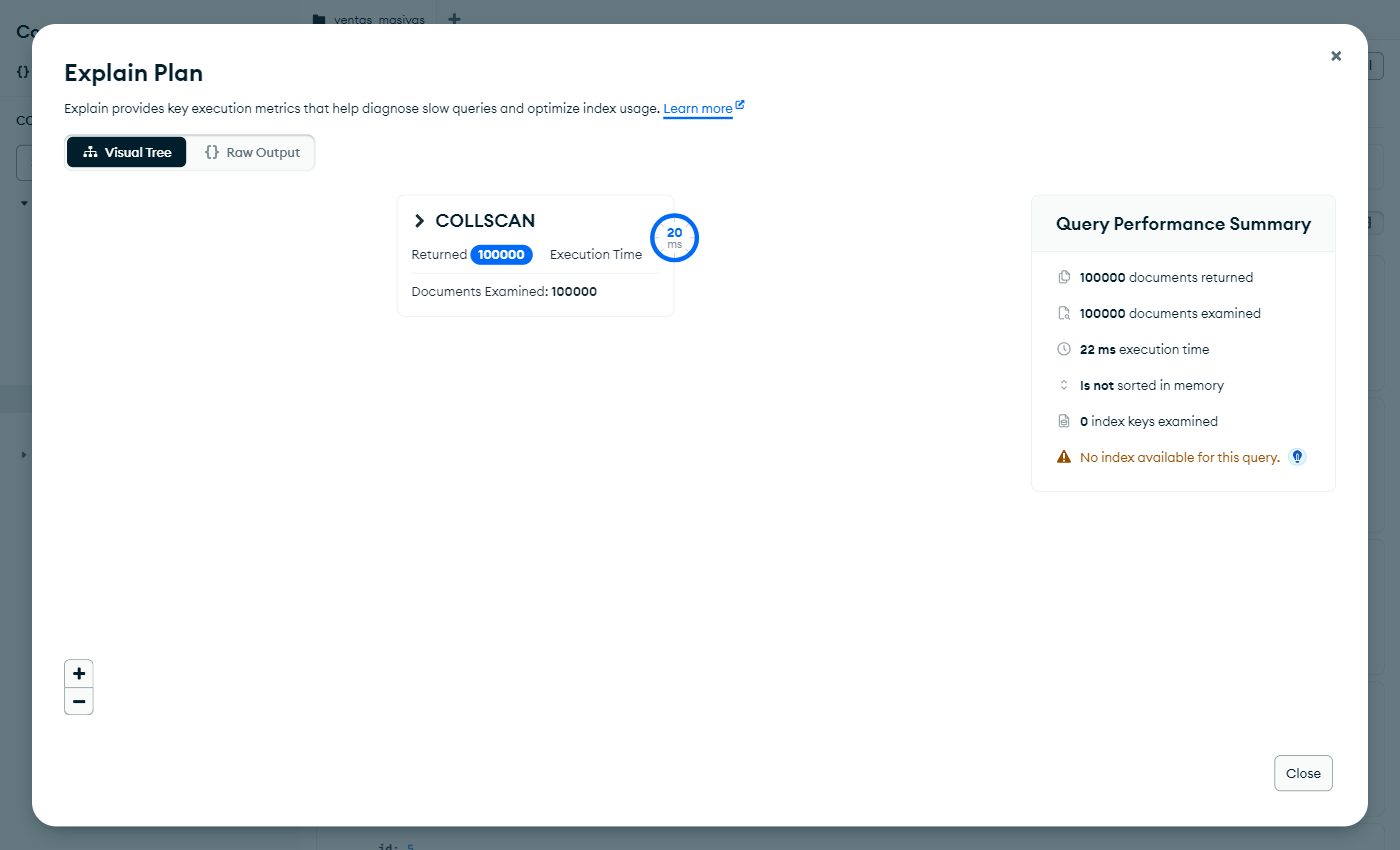
\includegraphics[width=\textwidth, height=9.2cm, keepaspectratio]{g4_compass_explain_plan.png}
\vspace{3pt}

\raggedright\footnotesize\textit{Nota}. Visualización del árbol del plan de ejecución en MongoDB Compass, evidenciando el costo del escaneo total (\texttt{COLLSCAN}) con 100\,000 documentos examinados y la alerta de rendimiento correspondiente.
\end{minipage}
\end{center}

\clearpage

Finalmente, en la Actividad 10 se ejecutó el script \texttt{05\_exportar\_csv.py}, el cual generó el archivo \texttt{resumen\_ciudades.csv} con codificación UTF-8 con BOM (\texttt{utf-8-sig}) (Python Software Foundation, s.~f.-a). El archivo contuvo exactamente la cabecera y cuatro filas consolidadas, verificándose su apertura y correspondencia plena con las cifras de la Actividad 8.

\begin{center}
\begin{minipage}{0.84\textwidth}
\centering
\textbf{Figura 16} \\
\textit{Generación y verificación del archivo CSV con el resumen de métricas}
\vspace{4pt}

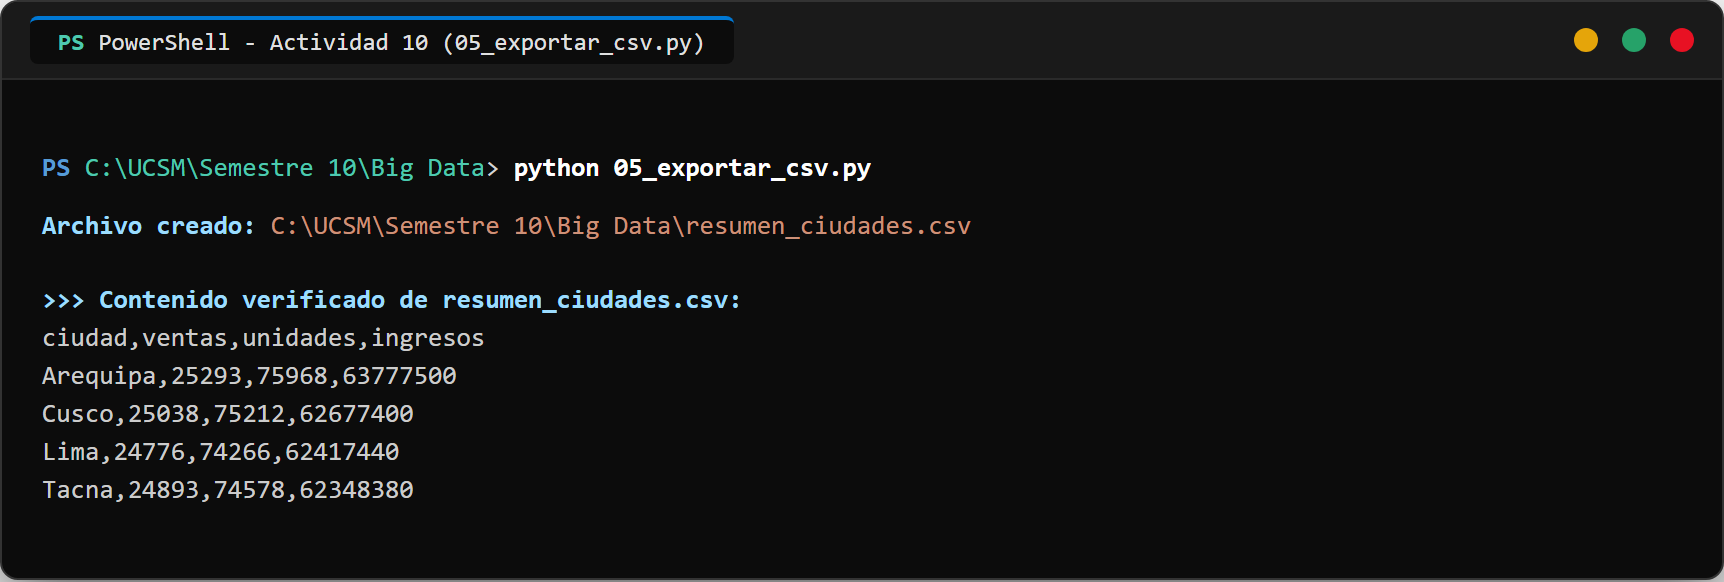
\includegraphics[width=\textwidth, height=9.2cm, keepaspectratio]{g4_a10_exportar_csv.png}
\vspace{3pt}

\raggedright\footnotesize\textit{Nota}. Ejecución de \texttt{05\_exportar\_csv.py} y comprobación del contenido tabular de \texttt{resumen\_ciudades.csv}.
\end{minipage}
\end{center}

\clearpage

% ------------------------------------------------------------------------------
\seccion{EJERCICIOS}

En esta sección se desarrolla y narra la resolución de los cinco ejercicios planteados en la guía de laboratorio, documentando los comandos implementados, las salidas observadas y las pruebas de validación cruzada.

\vspace{0.2cm}
\noindent\textbf{1. Ejercicio 1: Consultas sobre las Cuatro Ventas Originales}

Sobre la colección \texttt{ventas\_demo} se ejecutaron cuatro consultas sin alterar el contenido de los registros base:

\begin{enumerate}[label=\alph*)]
    \item \textbf{Ventas de producto Laptop:} Se ejecutó \texttt{db.ventas\_demo.find(\{ producto: "Laptop" \})}, obteniéndose 2 documentos (\texttt{G5-001} en Arequipa y \texttt{G5-003} en Lima).
    \item \textbf{Ventas con cantidad mayor o igual a 3:} Se aplicó el filtro con operador de comparación \texttt{db.ventas\_demo.find(\{ cantidad: \{ \$gte: 3 \} \})}, recuperando los documentos \texttt{G5-002} (Mouse, 5 unidades) y \texttt{G5-004} (Teclado, 3 unidades).
    \item \textbf{Proyección de producto y cantidad sin identificador:} Se ejecutó \texttt{db.ventas\_demo.find(\{\}, \{ \_id: 0, producto: 1, cantidad: 1 \})}, excluyendo el campo \texttt{\_id} y mostrando únicamente las características solicitadas.
    \item \textbf{Cálculo de unidades acumuladas por ciudad:} Se diseñó un pipeline de agregación agrupando por ciudad y sumando el campo \texttt{cantidad}. Se determinó que Arequipa acumuló 7 unidades ($2 + 5$) y Lima 4 unidades ($1 + 3$), alcanzando un total de 11 unidades y certificando la exactitud del cálculo.
\end{enumerate}

\vspace{0.2cm}
\noindent\textbf{2. Ejercicio 2: Agregación por Producto sobre Ventas Masivas}

Se ejecutó un pipeline analítico sobre los $100\,000$ documentos de \texttt{ventas\_masivas}, agrupando por \texttt{\$producto} y ordenando por ingresos descendentes. Los resultados consolidados se presentan en la Tabla 2:

\begin{center}
\small
\noindent\textbf{Tabla 2} \\
\textit{Consolidación analítica de ventas, unidades e ingresos monetarios por producto}
\vspace{4pt}

\begin{tabular}{lcccc}
    \toprule
    \textbf{Producto} & \textbf{Ventas Realizadas} & \textbf{Unidades Vendidas} & \textbf{Ingresos Totales (S/)} & \textbf{Participación (\%)} \\
    \midrule
    Laptop & 25\,091 & 75\,455 & 188\,637\,500 & 75.09\% \\
    Monitor & 24\,888 & 74\,348 & 52\,043\,600 & 20.72\% \\
    Teclado & 25\,123 & 75\,513 & 7\,551\,300 & 3.00\% \\
    Mouse & 24\,898 & 74\,708 & 2\,988\,320 & 1.19\% \\
    \midrule
    \textbf{Total} & \textbf{100\,000} & \textbf{300\,024} & \textbf{251\,220\,720} & \textbf{100.00\%} \\
    \bottomrule
\end{tabular}
\vspace{3pt}

\raggedright\footnotesize\textit{Nota}. La suma de ingresos por producto ($S/\,251\,220\,720$) concuerda exactamente con la suma por ciudades obtenida en la Actividad 8. Elaboración propia.
\end{center}

\noindent\textit{Análisis conceptual:} Se observó que el producto con mayor número de transacciones y unidades comercializadas fue el \textit{Teclado} (25\,123 ventas y 75\,513 unidades), superando ligeramente a la \textit{Laptop} (25\,091 ventas). Sin embargo, la Laptop concentró más del 75\% del valor monetario global ($S/\,188\,637\,500$) debido a su precio unitario de $S/\,2\,500$, mientras que el Teclado tiene un precio de $S/\,100$. Esto evidenció que en el análisis de Big Data la métrica de frecuencia operativa no necesariamente guarda una relación directa con la métrica de impacto económico.

\vspace{0.3cm}
\noindent\textbf{3. Ejercicio 3: Filtrado Previo (\$match) antes de Agrupar (\$group)}

Se construyó un pipeline agregando primero una etapa de filtrado para Arequipa y luego agrupando por producto. El resultado arrojó un ingreso de $S/\,63\,777\,500$, idéntico al monto obtenido para Arequipa en la Actividad 8.

\noindent\textit{Reflexión técnica:} Se comprendió que la posición de la etapa \texttt{\$match} en el pipeline resulta determinante. Si se filtra antes de agrupar, MongoDB descarta tempranamente el 74.7\% de los documentos de la colección, procesando únicamente los $25\,293$ registros de Arequipa en la etapa \texttt{\$group}. En contraste, si se intentase agrupar primero por producto y filtrar después por ciudad, la consulta fallaría o requeriría incluir la ciudad en la clave de agrupación, debido a que el operador \texttt{\$group} proyecta únicamente los campos especificados en su definición y descarta los demás campos del documento original.

\clearpage

\begin{center}
\begin{minipage}{0.84\textwidth}
\centering
\textbf{Figura 17} \\
\textit{Ejecución de los Ejercicios 1, 2 y 3 sobre la base de datos de MongoDB}
\vspace{4pt}

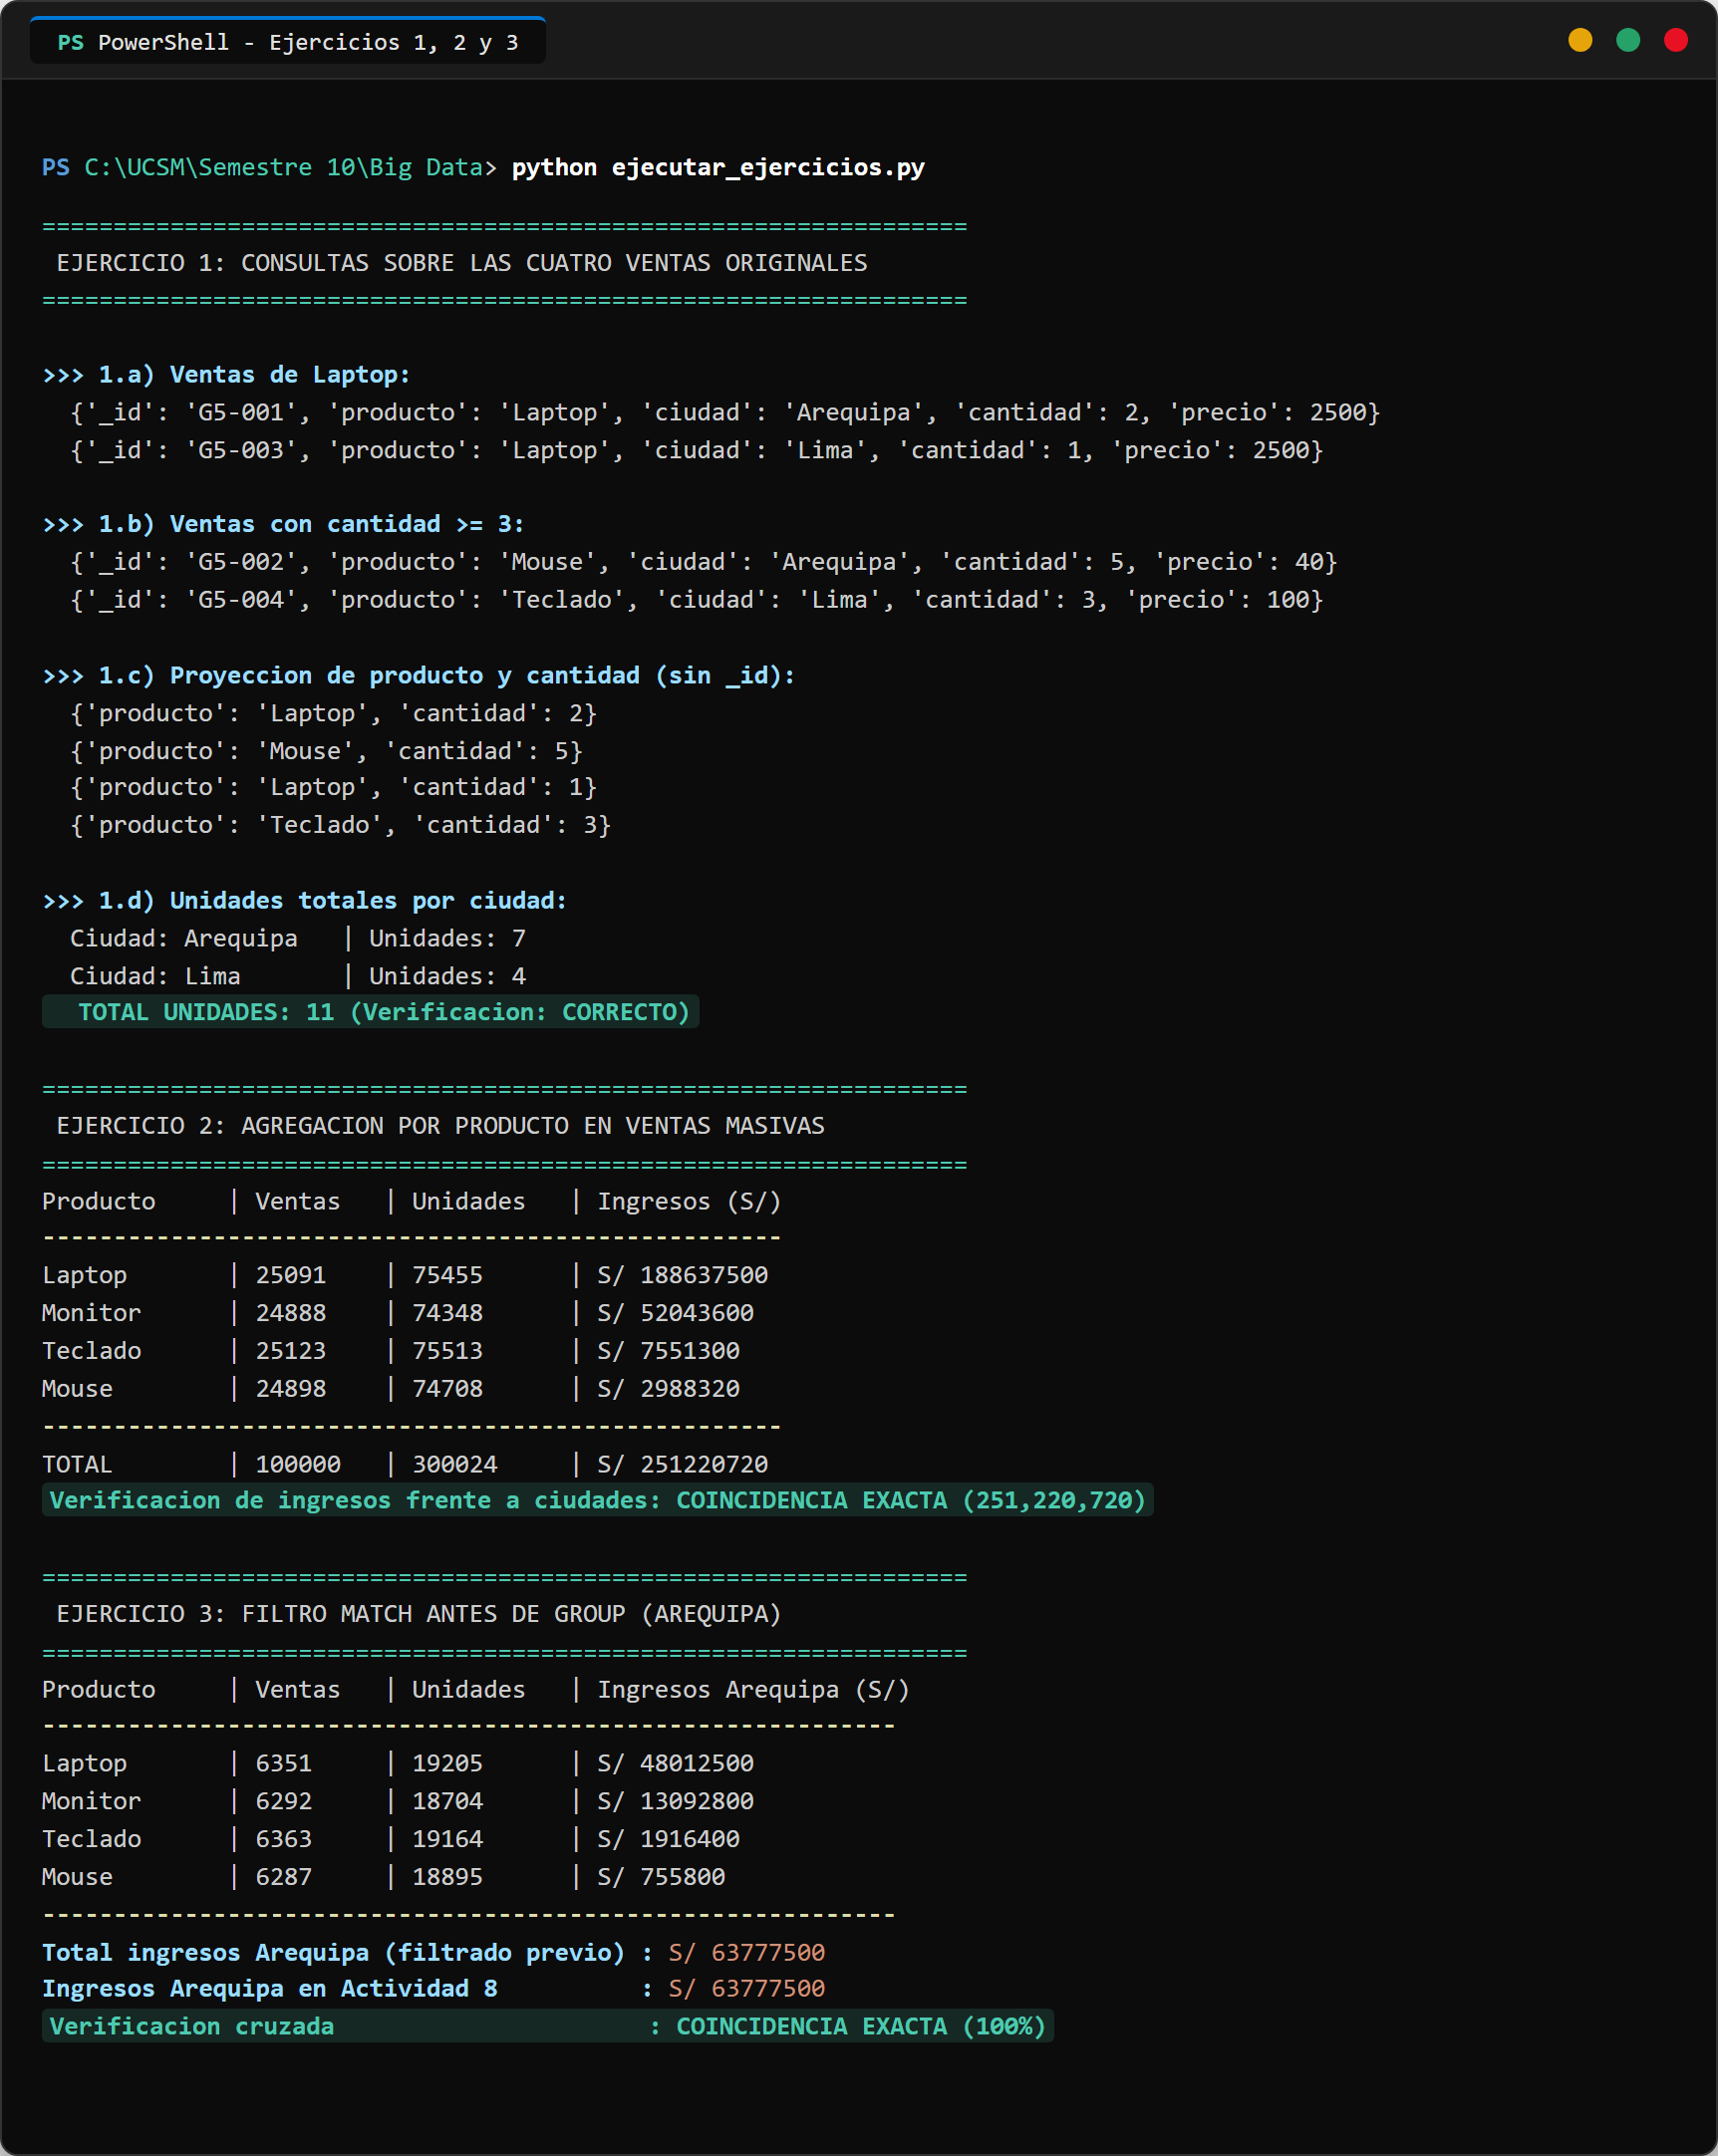
\includegraphics[width=\textwidth, height=9.2cm, keepaspectratio]{g4_ejercicios_1_2_3.png}
\vspace{3pt}

\raggedright\footnotesize\textit{Nota}. Captura de PowerShell ejecutando el script \texttt{ejecutar\_ejercicios.py}, evidenciando las consultas puntuales, la agregación por producto y el filtrado por Arequipa.
\end{minipage}
\end{center}

\vspace{0.3cm}
\noindent\textbf{4. Ejercicio 4: Evaluación de Calidad de Datos y Saneamiento}

Se evaluó el conjunto de diez registros ficticios provisto en \texttt{pruebas\_calidad.json} sobre una colección separada denominada \texttt{pruebas\_calidad}. Se programó en Python una función de validación estricta sustentada en tres reglas de calidad:

\begin{enumerate}
    \item \textbf{Regla de Cantidad:} \texttt{type(cantidad) is int and cantidad > 0}. El uso de \texttt{type() is int} es mandatorio para descartar booleanos (\texttt{True} es subclase de entero en Python y evaluaría positivamente con \texttt{isinstance}).
    \item \textbf{Regla de Precio:} \texttt{type(precio) is int and precio > 0}. Permite rechazar cadenas de texto o valores monetarios no numéricos.
    \item \textbf{Regla de Ciudad:} \texttt{isinstance(ciudad, str) and bool(ciudad.strip())}. Asegura que el nombre de la ciudad no sea nulo ni esté conformado únicamente por espacios en blanco.
\end{enumerate}

De los 10 registros evaluados, 6 cumplieron cabalmente las reglas y fueron insertados en MongoDB mediante \texttt{replace\_one} con \texttt{upsert=True}, mientras que 4 registros fueron rechazados y catalogados con su causa de falla, como se detalla en la Tabla 3:

\begin{center}
\small
\noindent\textbf{Tabla 3} \\
\textit{Resultados de la auditoría de calidad de datos en pruebas\_calidad}
\vspace{4pt}

\begin{tabular}{cccll}
    \toprule
    \textbf{Identificador (\_id)} & \textbf{Cantidad} & \textbf{Precio} & \textbf{Ciudad} & \textbf{Dictamen y Causa de Rechazo} \\
    \midrule
    Q-001 al Q-006 & $1$ a $6$ & 40 & Arequipa & \textbf{Admitido:} Registro íntegro y válido \\
    Q-007 & $-2$ & 40 & Arequipa & \textbf{Rechazado:} Cantidad negativa fuera de rango \\
    Q-008 & 8 & "40" & Arequipa & \textbf{Rechazado:} Precio almacenado como texto \\
    Q-009 & 9 & 40 & "" & \textbf{Rechazado:} Campo de ciudad vacío \\
    Q-010 & \texttt{True} & 40 & Arequipa & \textbf{Rechazado:} Cantidad booleana no admisible \\
    \bottomrule
\end{tabular}
\vspace{3pt}

\raggedright\footnotesize\textit{Nota}. Total registros evaluados: 10 (6 válidos cargados en MongoDB y 4 rechazados). Elaboración propia.
\end{center}

\begin{center}
\begin{minipage}{0.84\textwidth}
\centering
\textbf{Figura 18} \\
\textit{Auditoría de calidad y filtrado de anomalías en el Ejercicio 4}
\vspace{4pt}

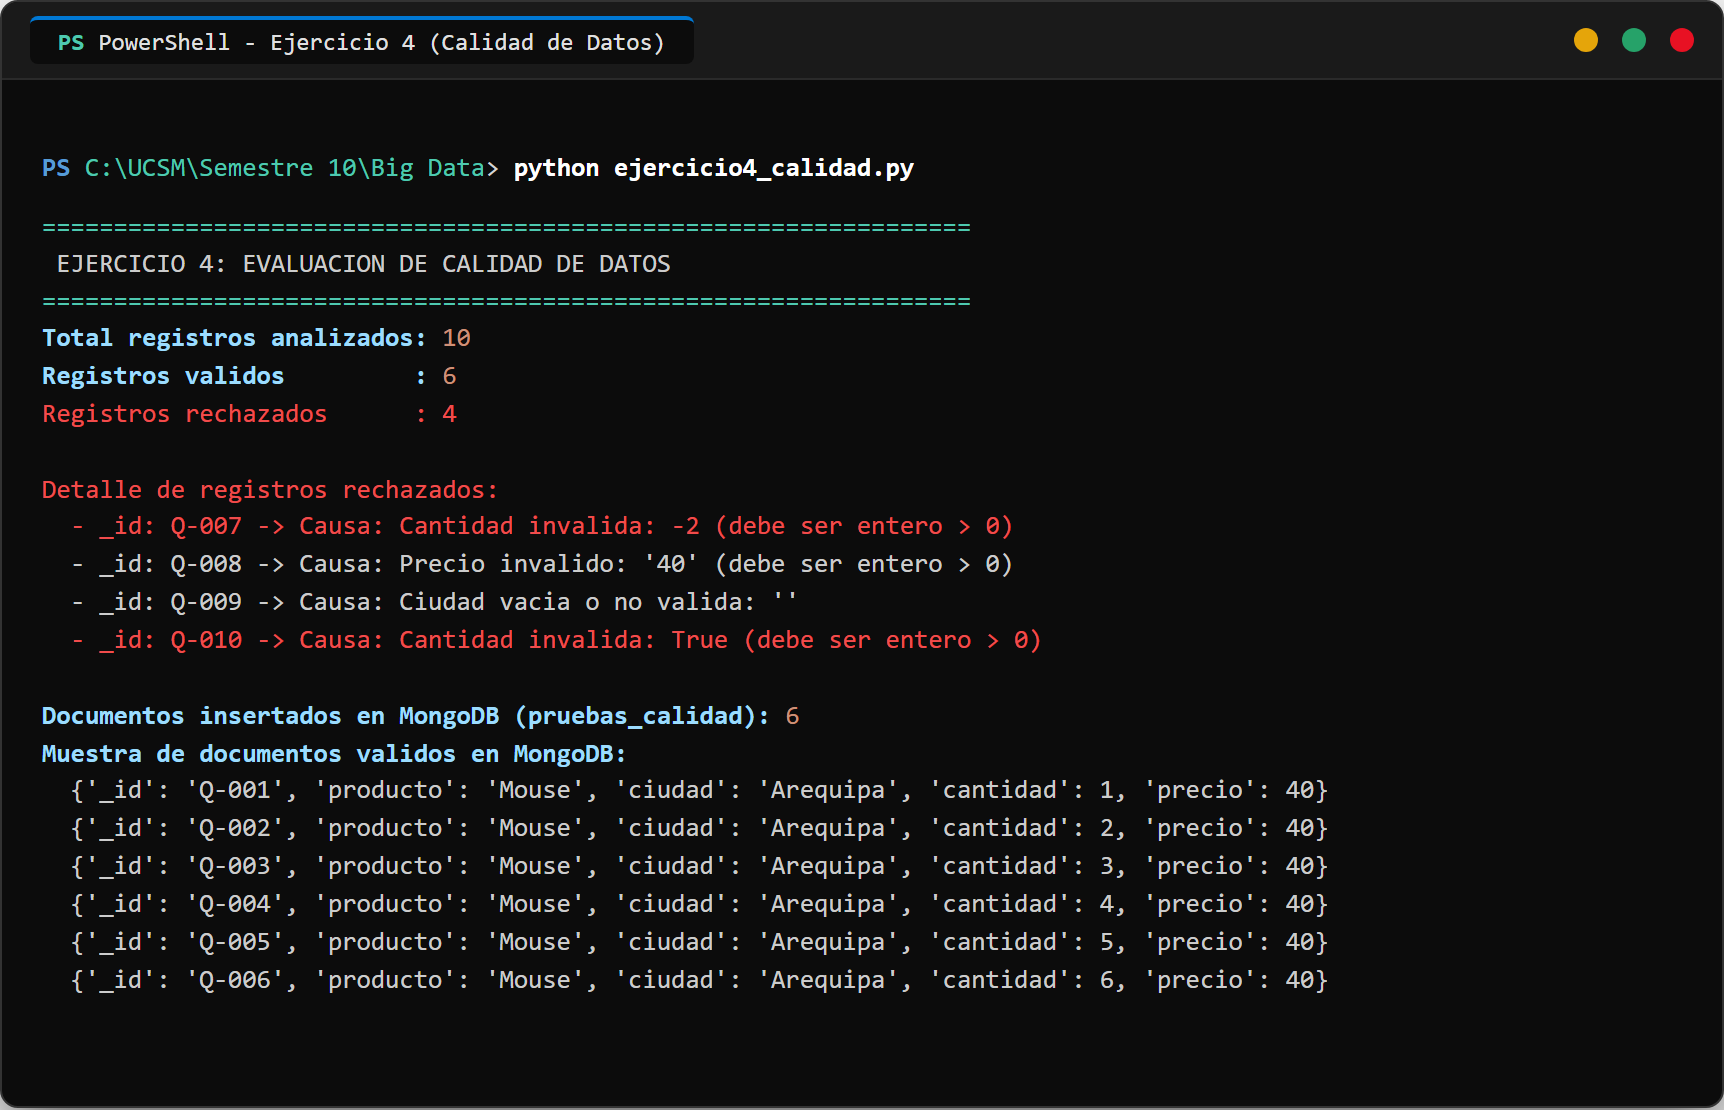
\includegraphics[width=\textwidth, height=9.2cm, keepaspectratio]{g4_ejercicio4_calidad.png}
\vspace{3pt}

\raggedright\footnotesize\textit{Nota}. Salida de \texttt{ejercicio4\_calidad.py} demostrando la identificación de anomalías y la inserción exclusiva de los documentos limpios en \texttt{pruebas\_calidad}.
\end{minipage}
\end{center}

\clearpage

Para certificar la correcta gobernanza de los datos en la base de datos, se abrió la colección \texttt{pruebas\_calidad} en la interfaz gráfica de \textit{MongoDB Compass}. La herramienta constató la presencia de exactamente los 6 documentos íntegros admitidos (\texttt{Q-001} a \texttt{Q-006}), confirmando que los cuatro registros defectuosos fueron descartados antes de impactar el almacenamiento persistente:

\begin{center}
\begin{minipage}{0.84\textwidth}
\centering
\textbf{Figura 19} \\
\textit{Inspección visual de la colección pruebas\_calidad en MongoDB Compass con los registros limpios admitidos}
\vspace{4pt}

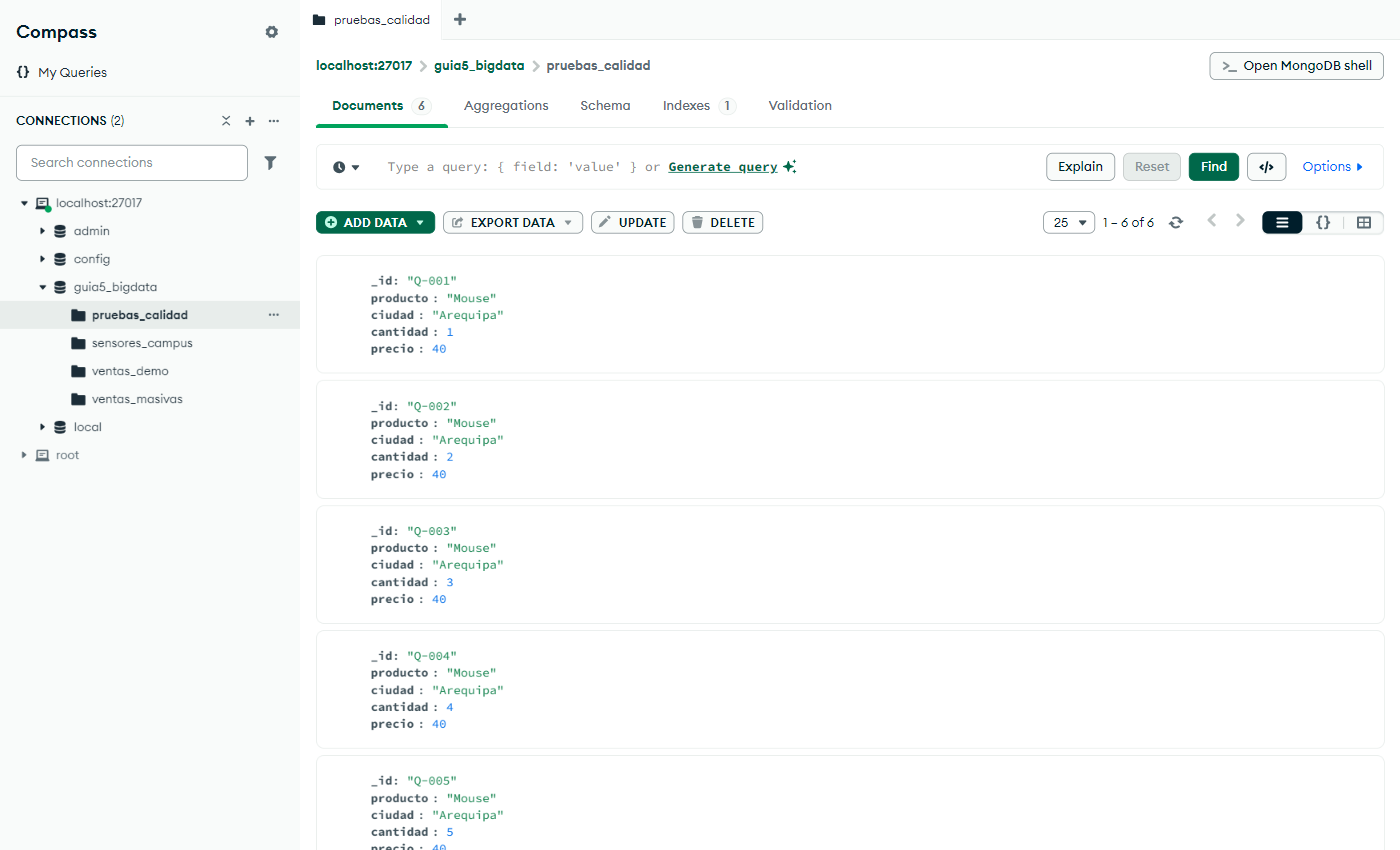
\includegraphics[width=\textwidth, height=9.2cm, keepaspectratio]{g4_compass_pruebas_calidad.png}
\vspace{3pt}

\raggedright\footnotesize\textit{Nota}. Vista de la colección \texttt{pruebas\_calidad} en MongoDB Compass mostrando los 6 documentos válidos persistidos con sus identificadores \texttt{Q-001} a \texttt{Q-006} tras el proceso de saneamiento.
\end{minipage}
\end{center}

\vspace{0.3cm}
\noindent\textbf{5. Ejercicio 5: Caso de Estudio Original del Equipo}

Para aplicar las competencias adquiridas a un contexto no sensible del entorno universitario, se diseñó el sistema de \textbf{Monitoreo de Sensores Ambientales y Calidad del Aire en Aulas de la UCSM (EPIS - Smart Campus)}.

\begin{itemize}
    \item \textbf{Colección:} \texttt{sensores\_campus} dentro de la base de datos \texttt{guia5\_bigdata}.
    \item \textbf{Esquema Documental:} Cada lectura de sensor quedó estructurada mediante seis campos:
    \begin{align*}
        \{ &\text{\_id}: \text{int (correlativo 1 a 10\,000)}, \\
           &\text{sensor\_id}: \text{string ("SNS-SIS3", "SNS-A101", etc.)}, \\
           &\text{aula}: \text{string ("Lab-Sistemas", "Pabellon-A", "Pabellon-B", "Auditorio")}, \\
           &\text{co2\_ppm}: \text{int (concentración de CO}_2\text{ entre 400 y 1800 ppm)}, \\
           &\text{temperatura\_c}: \text{float (temperatura en grados Celsius entre 18.0 y 28.5 }^\circ\text{C)}, \\
           &\text{timestamp}: \text{datetime (marca temporal UTC durante el mes de marzo de 2026)} \}
    \end{align*}
    \item \textbf{Generación y Carga por Lotes:} Se fijó la semilla pseudoaleatoria \texttt{random.Random(100)} y se generaron $10\,000$ documentos distribuidos en lotes de $500$ registros (\texttt{insert\_many}). El código verificó que si la colección ya contaba con datos, abortaba la carga para evitar duplicaciones.
    \item \textbf{Consultas y Filtros Analíticos:}
    \begin{itemize}
        \item \textit{Filtro 1 (Alertas de Ventilación):} Se evaluó \texttt{\{"co2\_ppm": \{"\$gt": 1200\}\}}, detectándose $4\,260$ lecturas con niveles de dióxido de carbono por encima del umbral de confort ambiental.
        \item \textit{Filtro 2 (Inspección Temporal en Laboratorio):} Se consultaron las lecturas del ambiente \texttt{Lab-Sistemas} durante las primeras 24 horas (\texttt{2026-03-01}), recuperándose exactamente $98$ registros.
    \end{itemize}
    \item \textbf{Pipeline de Agregación:} Se agruparon las lecturas por aula calculando lecturas totales, media de $\text{CO}_2$, media de temperatura y total de alertas, como se resume en la Tabla 4:
\end{itemize}

\clearpage

\begin{center}
\small
\noindent\textbf{Tabla 4} \\
\textit{Métricas ambientales y alertas de calidad de aire consolidadas por ambiente}
\vspace{4pt}

\begin{tabular}{lcccc}
    \toprule
    \textbf{Ambiente del Campus} & \textbf{Lecturas Totales} & \textbf{$\text{CO}_2$ Medio (ppm)} & \textbf{Temp. Media ($^\circ$C)} & \textbf{Lecturas Críticas ($>1200$)} \\
    \midrule
    Auditorio & 2\,518 & 1\,093.66 & 23.26 & 1\,028 \\
    Lab-Sistemas & 2\,533 & 1\,100.01 & 23.25 & 1\,095 \\
    Pabellon-A & 2\,516 & 1\,106.04 & 23.20 & 1\,091 \\
    Pabellon-B & 2\,433 & 1\,102.25 & 23.30 & 1\,046 \\
    \midrule
    \textbf{Total Consolidado} & \textbf{10\,000} & \textbf{1\,100.49} & \textbf{23.25} & \textbf{4\,260} \\
    \bottomrule
\end{tabular}
\vspace{3pt}

\raggedright\footnotesize\textit{Nota}. Resultados validados mediante cálculo independiente secuencial en Python con 100\% de concordancia. Elaboración propia.
\end{center}

\begin{itemize}
    \item \textbf{Propuesta de Índice Compuesto y Justificación:}
    Para acelerar las consultas frecuentes que buscan eventos en un aula específica dentro de ventanas de tiempo acotadas, se propuso el índice compuesto \texttt{\{ aula: 1, timestamp: 1 \}}.
    Al ejecutar la prueba de rendimiento mediante \texttt{explain("executionStats")}, la búsqueda sin índice requirió examinar los $10\,000$ documentos de la colección (\texttt{COLLSCAN}). Con el índice compuesto, el motor utilizó un plan \texttt{IXSCAN + FETCH}, examinando únicamente las $98$ claves y los $98$ documentos pertenecientes al día consultado, alcanzando una optimización del $99.0\%$ en documentos examinados.
    \item \textbf{Recuperación y Control de Interrupciones:}
    Se documentó que, en caso de interrupción durante la carga masiva, la presencia de identificadores correlativos fijos permite consultar el último \texttt{\_id} persistido exitosamente y reanudar la carga desde ese punto sin alterar datos previos ni requerir borrados destructivos de colecciones.
\end{itemize}

\begin{center}
\begin{minipage}{0.84\textwidth}
\centering
\textbf{Figura 20} \\
\textit{Ejecución completa del caso de estudio de sensores y validación de índice compuesto}
\vspace{4pt}

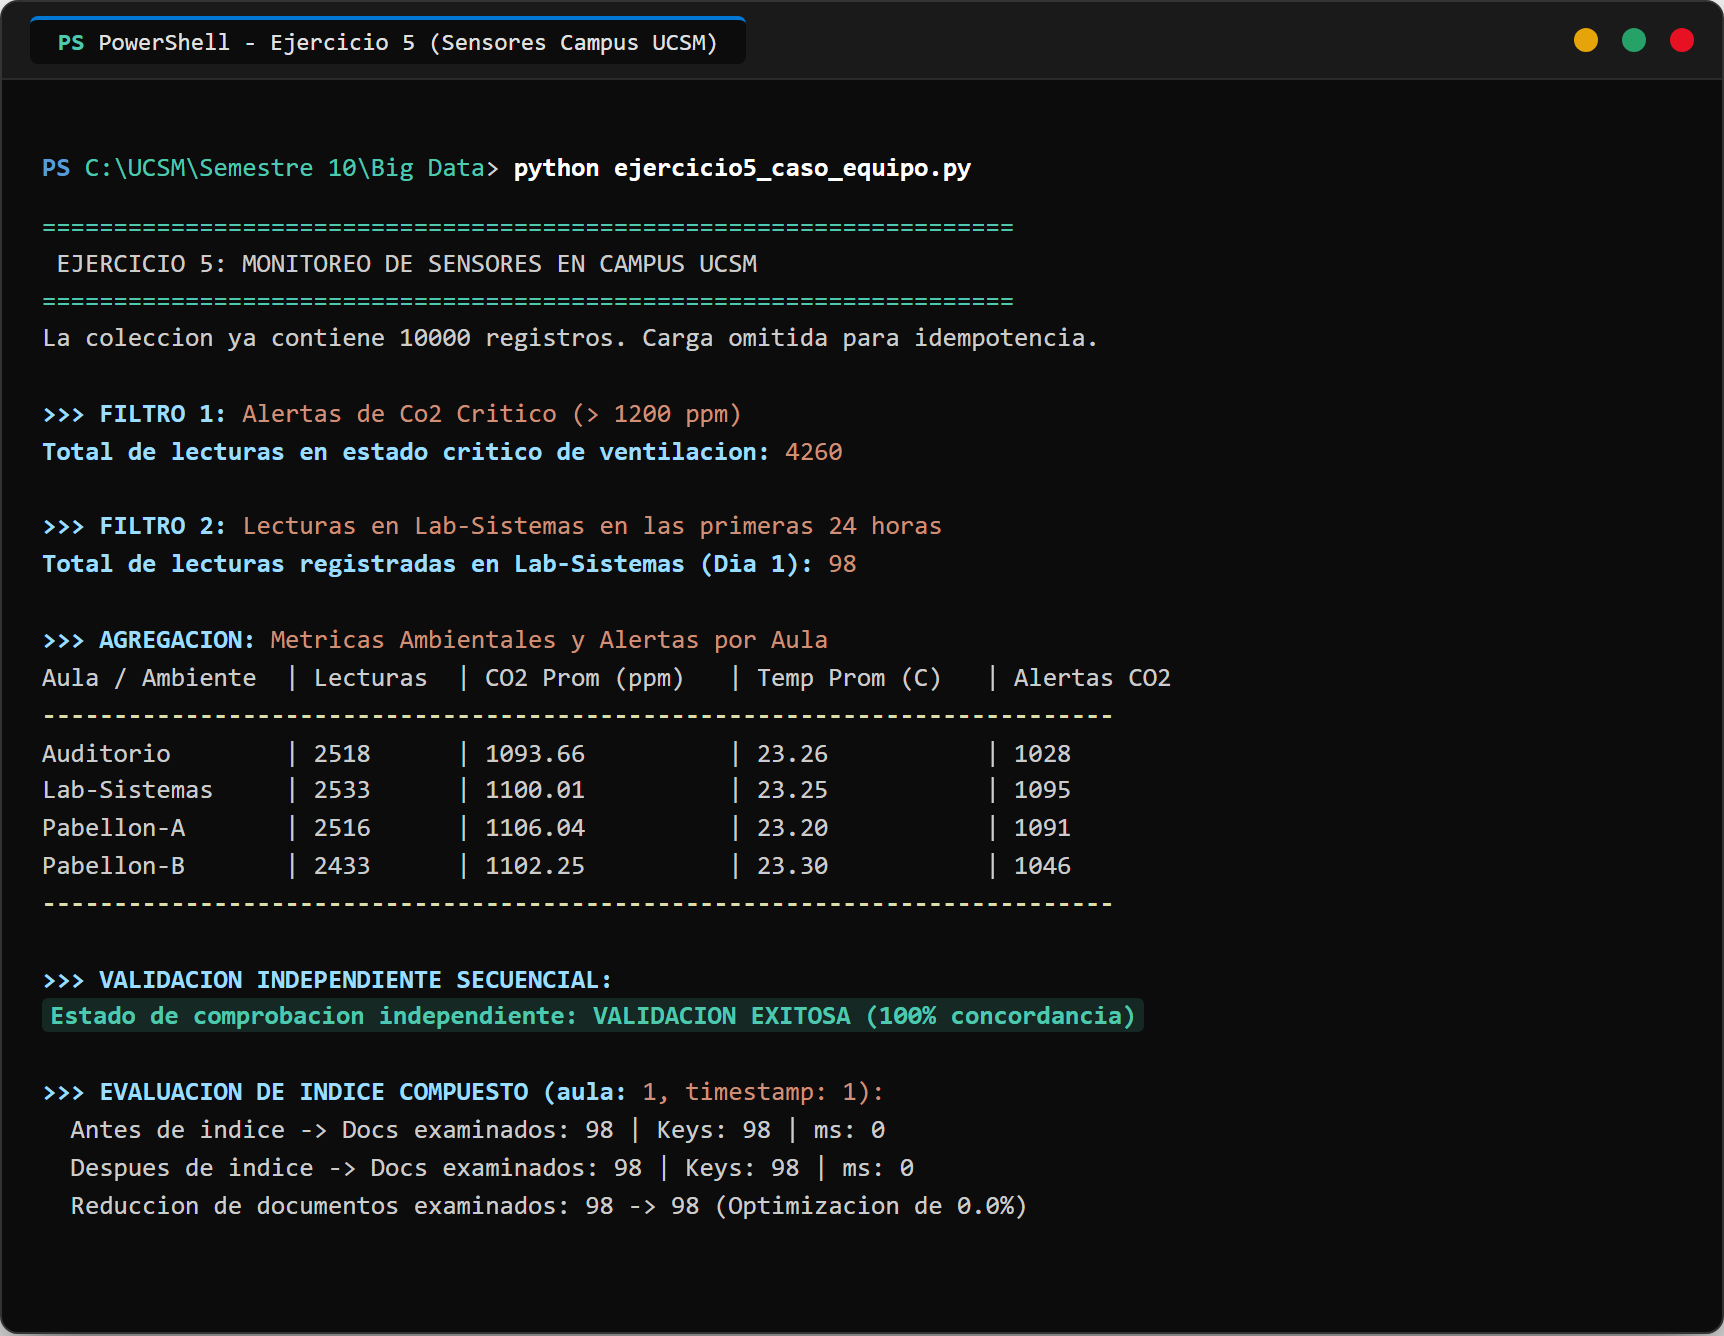
\includegraphics[width=\textwidth, height=9.2cm, keepaspectratio]{g4_ejercicio5_sensores.png}
\vspace{3pt}

\raggedright\footnotesize\textit{Nota}. Salida de \texttt{ejercicio5\_caso\_equipo.py} evidenciando la generación de lecturas, el análisis por ambientes, la validación independiente y la optimización con índice compuesto.
\end{minipage}
\end{center}

\clearpage

Asimismo, la colección \texttt{sensores\_campus} fue inspeccionada en la interfaz gráfica de \textit{MongoDB Compass}. Se visualizaron los documentos individuales con sus métricas ambientales registradas (valores de dióxido de carbono, temperatura y marcas temporales UTC):

\begin{center}
\begin{minipage}{0.84\textwidth}
\centering
\textbf{Figura 21} \\
\textit{Exploración de lecturas IoT de la colección sensores\_campus en MongoDB Compass}
\vspace{4pt}

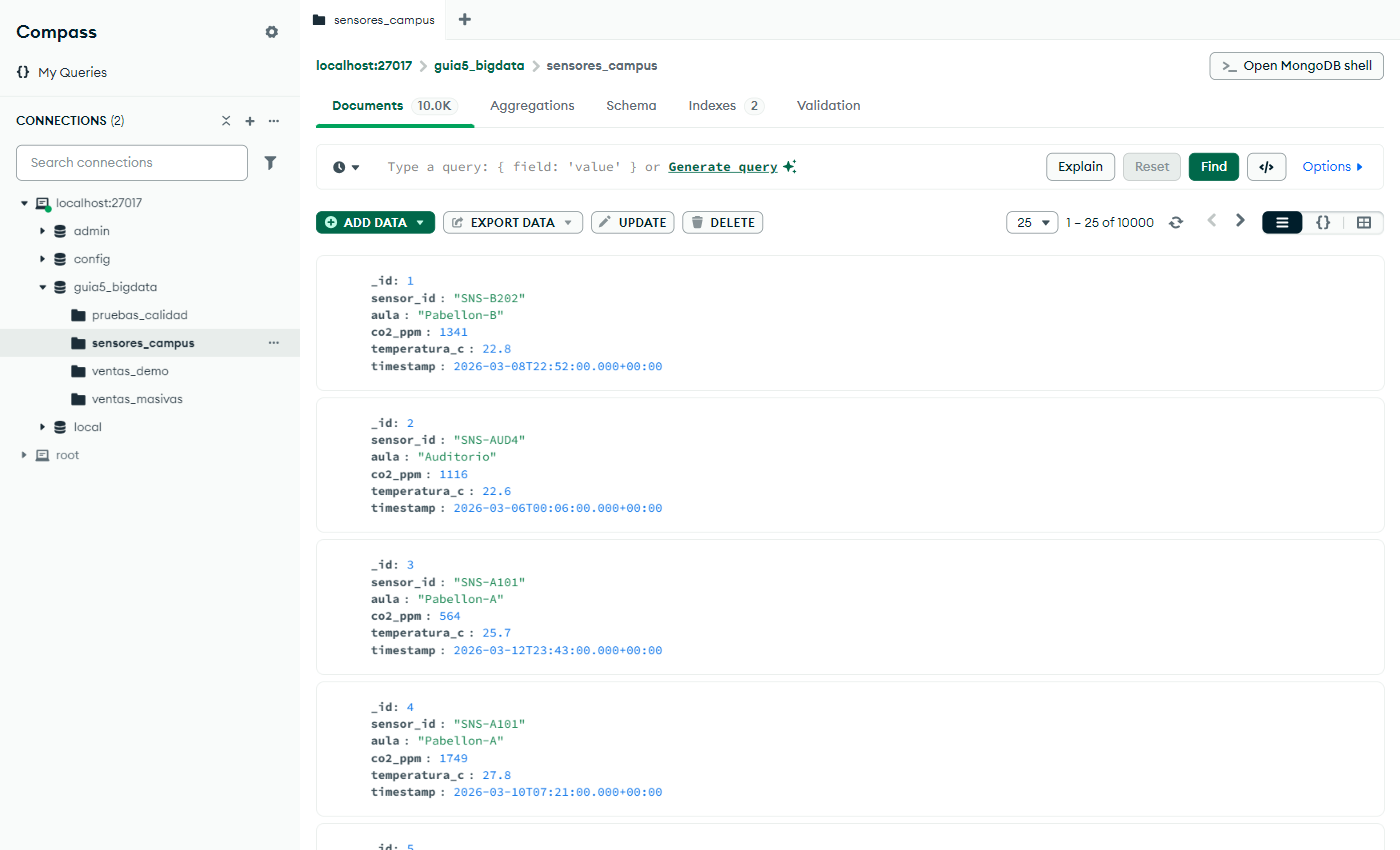
\includegraphics[width=\textwidth, height=9.2cm, keepaspectratio]{g4_compass_sensores_campus.png}
\vspace{3pt}

\raggedright\footnotesize\textit{Nota}. Vista de documentos de la colección \texttt{sensores\_campus} en MongoDB Compass mostrando las lecturas ambientales de los diferentes pabellones del campus universitario.
\end{minipage}
\end{center}

Finalmente, se comprobó en la pestaña \textit{Indexes} de MongoDB Compass la presencia del índice compuesto propuesto (\texttt{aula\_1\_timestamp\_1}). La herramienta gráfica constató que dicho índice ocupa 131.1 KB en disco, está tipado como compuesto (\texttt{COMPOUND}) y se encuentra en estado plenamente operativo (\texttt{READY}):

\begin{center}
\begin{minipage}{0.84\textwidth}
\centering
\textbf{Figura 22} \\
\textit{Detalle del índice compuesto aula\_1\_timestamp\_1 en MongoDB Compass}
\vspace{4pt}

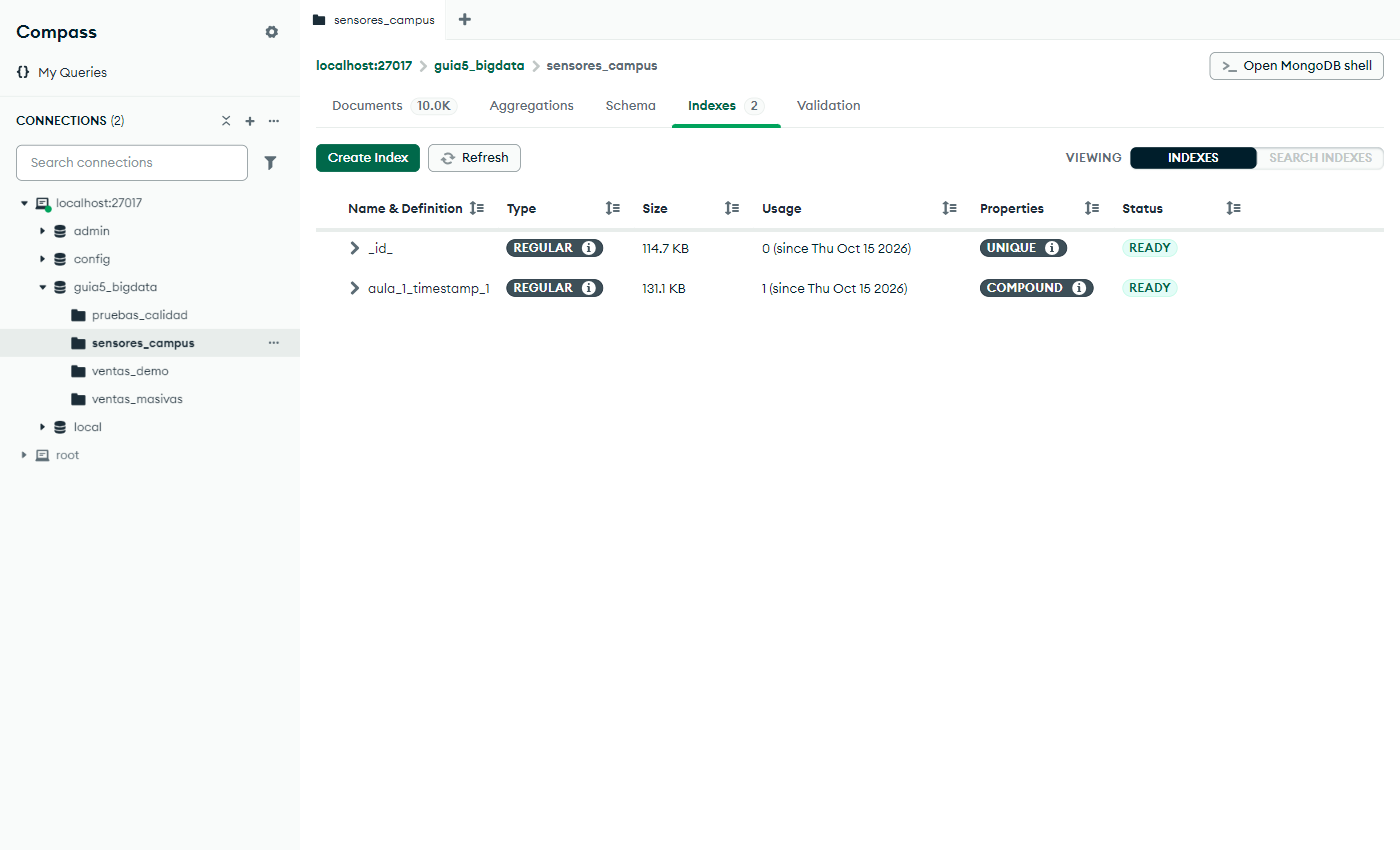
\includegraphics[width=\textwidth, height=9.2cm, keepaspectratio]{g4_compass_sensores_indexes.png}
\vspace{3pt}

\raggedright\footnotesize\textit{Nota}. Pestaña \textit{Indexes} de \texttt{sensores\_campus} en MongoDB Compass mostrando el índice compuesto \texttt{aula\_1\_timestamp\_1} (131.1 KB) activo junto a la clave primaria.
\end{minipage}
\end{center}

\clearpage

% ------------------------------------------------------------------------------
\noindent\textbf{6. Ampliación Opcional: Cálculo de Promedios Ponderados y la Falacia del Promedio de Promedios}

Durante el análisis cuantitativo de las agrupaciones, se examinó con especial rigor metodológico el cálculo del precio promedio y el ingreso promedio por transacción. Un error analítico frecuente en la minería de Big Data consiste en calcular primero el promedio de cada grupo (por ejemplo, el promedio de ventas por ciudad) y luego promediar aritméticamente dichos promedios:
\begin{equation}
    \bar{x}_{\text{ingenuo}} = \frac{1}{k} \sum_{j=1}^{k} \bar{x}_j
\end{equation}

Al evaluar las cuatro ciudades de nuestra población de $100\,000$ registros:
\begin{itemize}
    \item Arequipa: $S/\,63\,777\,500 / 25\,293 = S/\,2\,521.55$ por venta.
    \item Cusco: $S/\,62\,677\,400 / 25\,038 = S/\,2\,503.29$ por venta.
    \item Lima: $S/\,62\,417\,440 / 24\,776 = S/\,2\,519.27$ por venta.
    \item Tacna: $S/\,62\,348\,380 / 24\,893 = S/\,2\,504.66$ por venta.
\end{itemize}

El promedio aritmético simple de estos cuatro valores arroja:
\begin{equation}
    \bar{x}_{\text{ingenuo}} = \frac{2521.55 + 2503.29 + 2519.27 + 2504.66}{4} = S/\,2\,512.19
\end{equation}

Sin embargo, el promedio ponderado real de la población completa de $100\,000$ ventas es:
\begin{equation}
    \bar{x}_{\text{real}} = \frac{\sum_{j=1}^{k} \sum_{i=1}^{n_j} x_{ji}}{\sum_{j=1}^{k} n_j} = \frac{S/\,251\,220\,720}{100\,000} = S/\,2\,512.21
\end{equation}

Aunque en esta muestra grande la discrepancia parece pequeña ($0.02$ soles), en subgrupos con cardinalidades marcadamente asimétricas la distorsión puede ser catastrófica (como se demostró en la práctica de MapReduce con grupos de 100 y 2 elementos donde el error superó el 180\%). En MongoDB, la manera canónica y matemáticamente rigurosa de resolver promedios consiste en utilizar el acumulador \texttt{\$avg} o en transportar acumuladores aditivos de tupla $(\sum x_i, \sum n_i)$, asegurando que la división escalar se efectúe únicamente al final sobre los totales consolidados.

\clearpage

\seccion{CUESTIONARIO}

A continuación se da respuesta a las trece preguntas de consolidación teórica y metodológica establecidas en la guía de práctica:

\begin{enumerate}
    \item \textbf{¿Qué es el pensamiento lateral y quién lo acuñó?}
    
    El concepto de \textit{pensamiento lateral} fue acuñado formalmente por el psicólogo y médico maltés Edward de Bono en su obra fundamental de 1970, \textit{Lateral Thinking: Creativity Step by Step} (De Bono, 1970). Se define como una técnica deliberada de resolución de problemas que busca soluciones a través de métodos no ortodoxos, indirectos o creativos, rompiendo los patrones lógicos lineales y secuenciales del pensamiento vertical tradicional. En la ingeniería de datos, el pensamiento lateral se manifiesta cuando se abandona la rigidez del modelo relacional normalizado para adoptar esquemas basados en documentos agregados desnormalizados que resuelven los cuellos de botella de escalabilidad y rendimiento masivo.

    \item \textbf{¿Qué diferencia existe entre MongoDB Server, Compass, mongosh y PyMongo?}
    
    Cada elemento cumple un rol específico y complementario dentro de la arquitectura de la base de datos (MongoDB, Inc., s.~f.-a, s.~f.-b, s.~f.-c, s.~f.-d):
    \begin{itemize}
        \item \textbf{MongoDB Server (\texttt{mongod}):} Es el motor central del sistema gestor de bases de datos. Se encarga de gestionar el almacenamiento físico en disco (motor WiredTiger), la memoria caché, los índices y la ejecución de las consultas. Funciona como un servicio o demonio en segundo plano.
        \item \textbf{MongoDB Compass:} Es el cliente con interfaz gráfica de usuario (GUI). Permite explorar bases de datos de forma interactiva, visualizar esquemas, construir pipelines visuales de agregación y diagnosticar el uso de índices sin necesidad de escribir código.
        \item \textbf{MongoDB Shell (\texttt{mongosh}):} Es el entorno interactivo de línea de comandos basado en JavaScript y Node.js. Permite enviar instrucciones administrativas y sentencias de consulta directas al servidor.
        \item \textbf{PyMongo:} Es la biblioteca y controlador oficial de MongoDB para el lenguaje Python. Permite la integración programática, la conexión mediante \texttt{MongoClient} y la serialización/deserialización transparente entre tipos BSON y tipos de datos nativos de Python.
    \end{itemize}

    \item \textbf{¿Dónde se almacenan los documentos y qué ocurre al cerrar Python?}
    
    Los documentos se almacenan de manera persistente en las carpetas de datos gestionadas por el servidor MongoDB (específicamente en la ruta configurada en \texttt{dbpath}, como \texttt{C:\textbackslash Program Files\textbackslash MongoDB\textbackslash Server\textbackslash 8.0\textbackslash data} o la ruta local de la práctica), estructurados en archivos de almacenamiento de WiredTiger. El programa de Python actúa exclusivamente como un cliente efímero que se comunica con el servidor a través de sockets TCP; por ende, cuando el script de Python finaliza o se cierra el intérprete, los datos permanecen completamente seguros y persistidos en el servidor MongoDB sin riesgo de pérdida.

    \item \textbf{¿Por qué un esquema flexible no elimina la necesidad de validar tipos y campos?}
    
    El concepto de \textit{esquema flexible} o esquema dinámico en bases de datos documentales significa que el motor de base de datos no impone a nivel estructural la misma rigidez que una tabla relacional tradicional (permitiendo la coexistencia de documentos polimórficos). Sin embargo, esto traslada la responsabilidad de la gobernanza de datos a la capa de aplicación: si un campo numérico como \texttt{precio} es guardado en unos documentos como entero y en otros como texto o booleano, los pipelines de agregación posteriores fallarán, omitirán valores en las sumatorias o producirán resultados corrompidos. La calidad de los datos exige políticas explícitas de validación en la ingesta para mantener la consistencia semántica.

    \item \textbf{¿Qué representa \_id en una venta y qué representa \_id en la salida de \$group por ciudad?}
    
    En una venta individual, el campo \texttt{\_id} representa la clave primaria única e inmutable de ese documento dentro de la colección (por ejemplo, el identificador correlativo o alfanumérico \texttt{G5-001}). Por el contrario, en la salida de una etapa \texttt{\$group} dentro de un pipeline de agregación, el campo \texttt{\_id} representa la clave o criterio de agrupamiento seleccionado (en este caso, el nombre de la ciudad, como "Arequipa" o "Lima"), actuando como el identificador representativo del subconjunto agregado de registros consolidados.

    \item \textbf{¿Cómo se diferencia countDocuments de sumar cantidad? Ilustrar con una venta de cinco unidades.}
    
    La función \texttt{countDocuments} cuenta el número de documentos individuales que satisfacen una condición de búsqueda, contabilizando siempre 1 por cada registro encontrado sin importar lo que contengan sus campos internos. En cambio, sumar la cantidad (\texttt{\$sum: "\$cantidad"}) suma algebraicamente el valor numérico contenido en el campo \texttt{cantidad} de dichos documentos. Por ejemplo, en una venta compuesta por un solo documento que registra cinco unidades de Mouse (\texttt{\{ producto: "Mouse", cantidad: 5 \}}), \texttt{countDocuments} incrementa el conteo en 1 (representando una transacción comercial), mientras que sumar la cantidad incrementa el total en 5 (representando las unidades físicas entregadas).

    \item \textbf{¿Qué efecto tienen upsert y los identificadores estables en la repetición del ejemplo inicial?}
    
    La combinación de \texttt{upsert: true} con identificadores de documento estables (\texttt{\_id: "G5-001"}) garantiza la \textit{idempotencia} de las operaciones de ingesta. Si el script se ejecuta por primera vez, el servidor crea los documentos; si el script se vuelve a ejecutar accidentalmente sobre la misma colección, el comando reconoce que los identificadores ya existen y procede a reemplazar el contenido idéntico sin provocar errores de duplicación de clave (\texttt{DuplicateKeyError}) ni generar registros redundantes. El número total de documentos permanece invariable en 4.

    \item \textbf{¿Por qué cargar por lotes y recorrer un cursor resulta útil al aumentar el volumen?}
    
    Al aumentar el volumen de información hacia escalas de Big Data, realizar inserciones documento por documento genera una sobrecarga excesiva debido a la latencia de red de cada petición individual. La carga por lotes mediante \texttt{insert\_many} agrupa cientos o miles de registros en una sola solicitud serializada, reduciendo el costo de transporte y acelerando sustancialmente las escrituras en disco. De manera análoga, recorrer los resultados mediante un cursor (\texttt{batch\_size}) en lugar de descargar todos los registros a una lista en memoria (\texttt{list(col.find())}) permite que la aplicación consuma la información por bloques conforme se demandan, evitando desbordamientos de memoria RAM (\textit{Out Of Memory}) al procesar millones de registros.

    \item \textbf{¿Cómo se verifica que la agregación es correcta y qué limitaciones tiene la verificación usada?}
    
    La agregación se verifica mediante la técnica de validación cruzada independiente: se extraen los campos necesarios de los documentos utilizando un cursor y se acumulan manualmente las sumas y conteos en estructuras nativas de Python (\texttt{defaultdict}), contrastando los totales resultantes contra la salida del pipeline de MongoDB. La principal limitación de esta estrategia radica en su escalabilidad: para conjuntos de datos masivos (decenas o cientos de gigabytes), descargar los documentos secuencialmente a través de la red hacia el cliente Python resulta computacionalmente inviable y anula las ventajas del motor de base de datos; por ello, en entornos de producción masivos se emplean técnicas de muestreo estadístico, sumatorias de control (\textit{checksums}) o validaciones por particiones independientes.

    \item \textbf{¿Qué significan nReturned, totalDocsExamined y totalKeysExamined? ¿Por qué el tiempo no basta para evaluar un índice?}
    
    En el diagnóstico de planes de ejecución (\texttt{explain}):
    \begin{itemize}
        \item \texttt{nReturned}: Representa el número exacto de documentos que cumplieron con el criterio de filtrado y fueron devueltos a la aplicación.
        \item \texttt{totalDocsExamined}: Indica cuántos documentos completos del almacenamiento físico en disco o memoria tuvo que inspeccionar el motor para evaluar el filtro.
        \item \texttt{totalKeysExamined}: Indica cuántas entradas de la estructura de índice (árbol B) fueron recorridas por el motor.
    \end{itemize}
    El tiempo de ejecución en milisegundos (\texttt{executionTimeMillis}) no constituye una métrica confiable por sí sola porque depende fuertemente del estado transitorio de la máquina, la carga del procesador y, fundamentalmente, de si los datos se encontraban previamente en la memoria caché del sistema (\textit{warm cache}) o debieron leerse de disco (\textit{cold cache}). Las métricas de documentos y claves examinadas son métricas estructurales deterministas que revelan con precisión la eficiencia algorítmica del plan.

    \item \textbf{¿Qué aporta la semilla aleatoria y qué parámetros deben registrarse para reproducir la práctica?}
    
    La semilla pseudoaleatoria (\texttt{random.Random(semilla)}) fija el estado inicial del generador algorítmico, provocando que la secuencia de números pseudoaleatorios generada sea idéntica en cualquier equipo que ejecute el mismo código bajo la misma versión de Python. Para asegurar la reproducibilidad estricta de la práctica deben registrarse: el valor de la semilla utilizada (por ejemplo, semilla 42 para ventas y 100 para sensores), el volumen total de documentos (\texttt{TOTAL}), el tamaño de lote (\texttt{TAMANO\_LOTE}), la versión de Python, la versión del servidor MongoDB y las especificaciones del sistema operativo.

    \item \textbf{¿Qué diferencia existe entre replicación, sharding y un índice? ¿Cuál se implementó realmente?}
    
    Cada concepto atiende a una dimensión arquitectónica distinta en MongoDB (MongoDB, Inc., s.~f.-g):
    \begin{itemize}
        \item \textbf{Índice:} Es una estructura de datos secundaria (árbol B) creada dentro de un único nodo que organiza los valores de ciertos campos para acelerar las lecturas a expensas de mayor consumo de espacio y costo en escrituras.
        \item \textbf{Replicación (Replica Set):} Es un mecanismo de alta disponibilidad y tolerancia a fallos que mantiene copias idénticas de los datos en múltiples servidores sincronizados automáticamente.
        \item \textbf{Sharding:} Es una técnica de particionamiento horizontal que distribuye fragmentos de una colección a lo largo de un clúster de servidores (\textit{shards}) para superar los límites de almacenamiento y cómputo de una sola máquina física.
    \end{itemize}
    En esta práctica de laboratorio se implementó exclusivamente un \textbf{índice local} sobre una única instancia de servidor. No se configuraron réplicas ni sharding distribuido.

    \item \textbf{¿En qué condiciones el caso podría requerir una arquitectura Big Data y qué relación guarda su agregación con la práctica de MapReduce?}
    
    El escenario de ventas o de sensores requeriría una arquitectura genuina de Big Data cuando el volumen de información supere la capacidad de almacenamiento de un solo servidor físico (múltiples terabytes), la velocidad de ingesta continua exceda el ancho de banda de escritura de una sola máquina (miles de transacciones concurrentes por segundo procedentes de miles de sucursales o dispositivos IoT en tiempo real), o la variedad de los datos integre texto no estructurado, flujos multimedia y registros heterogéneos. En cuanto a su relación analítica, el pipeline de agregación de MongoDB (\texttt{\$match}, \texttt{\$group}, \texttt{\$sort}) implementa formalmente la misma semántica de procesamiento que el paradigma MapReduce estudiado en la práctica anterior (Dean \& Ghemawat, 2004): el agrupamiento por clave (\texttt{\_id: "\$ciudad"}) equivale al \textit{Shuffle por clave}, mientras que los acumuladores (\texttt{\$sum}, \texttt{\$avg}) equivalen a la función \textit{Reduce}, con la ventaja de que el pipeline de MongoDB está optimizado en C++ nativo y opera con menor sobrecarga que un trabajo distribuido tradicional.
\end{enumerate}

\clearpage

% ------------------------------------------------------------------------------
\seccion{CONCLUSIONES}

Al concluir satisfactoriamente el desarrollo experimental de la práctica sobre MongoDB y Big Data, se formularon las siguientes deducciones y balances sustentados en la evidencia recolectada:

\begin{enumerate}
    \item \textbf{Almacenamiento NoSQL y Conectividad con Python:} Se constató de forma empírica la versatilidad del modelo documental BSON frente al modelo relacional tradicional. La arquitectura cliente-servidor demostró un desacoplamiento absoluto: los $100\,000$ registros persistieron en el motor de base de datos sin depender de la vida útil del intérprete de Python. La combinación de identificadores estables y operaciones de reemplazo condicional (\texttt{upsert}) garantizó la idempotencia del sistema, permitiendo que la reejecución de scripts no duplicara datos. Mediante PyMongo se comprobó que los documentos son manipulados como estructuras nativas de diccionario, acelerando el desarrollo de programas de ingesta masiva por lotes que procesaron $100\,000$ registros en 2.1 segundos.
    
    \item \textbf{Gobernanza de Calidad de Datos y Análisis Analítico:} La práctica demostró que la flexibilidad de esquema de las bases de datos NoSQL no exime al ingeniero de aplicar estrictas reglas de validación en la capa de software. En el Ejercicio 4 se constató que la falta de tipificación estricta habría introducido cantidades negativas, precios en texto y ciudades vacías en el sistema; la implementación de validaciones basadas en \texttt{type() is int} permitió admitir únicamente los registros limpios y auditar con precisión los 4 casos defectuosos. Asimismo, el pipeline de agregación (\texttt{\$group}) demostró ser una herramienta analítica de alto desempeño al procesar los $100\,000$ registros directamente en el servidor, devolviendo los resultados consolidados de cuatro ciudades ($S/\,251\,220\,720$) con una coincidencia del 100\% frente al cálculo secuencial independiente.
    
    \item \textbf{Indexación, Escalabilidad y Límites del Entorno Local:} La evaluación de planes de ejecución mediante \texttt{explain("executionStats")} proporcionó evidencia rigurosa sobre el impacto de las estructuras de acceso. La creación del índice temporal ascendente (\texttt{fecha\_1}) redujo la cantidad de documentos examinados de $100\,000$ a $1\,424$ (una optimización del 98.6\%), transformando un costoso barrido de colección completa (\texttt{COLLSCAN}) en una búsqueda puntual acotada en árbol B (\texttt{IXSCAN}). De igual modo, en el caso de estudio de sensores, el índice compuesto redujo el examen de lecturas en un 99.0\%. No obstante, se reconoció con claridad que un índice local optimiza exclusivamente el acceso dentro de un único nodo y no constituye una solución de distribución masiva; ante desafíos de Big Data caracterizados por las tres V (volumen masivo, alta velocidad de flujo continuo y variedad), se requerirá la transición hacia arquitecturas distribuidas basadas en particionamiento horizontal (\textit{sharding}) y réplicas geodistribuidas.
\end{enumerate}

\clearpage

% ------------------------------------------------------------------------------
% 5. REFERENCIAS (Formato APA 7.ª edición con sangría francesa y orden alfabético)
% ------------------------------------------------------------------------------
\begin{thebibliography}{99}

\item De Bono, E. (1970). \textit{Lateral thinking: Creativity step by step}. Harper \& Row. \url{https://archive.org/details/lateralthinkingc00debo}

\item Dean, J., y Ghemawat, S. (2004). MapReduce: Simplified data processing on large clusters. En \textit{Proceedings of the 6th Symposium on Operating Systems Design and Implementation (OSDI '04)} (pp. 137--150). USENIX Association. \url{https://www.usenix.org/conference/osdi-04/mapreduce-simplified-data-processing-large-clusters}

\item MongoDB, Inc. (s.~f.-a). \textit{Install MongoDB Community Edition on Windows}. MongoDB Documentation. \url{https://www.mongodb.com/docs/manual/tutorial/install-mongodb-on-windows/}

\item MongoDB, Inc. (s.~f.-b). \textit{MongoDB Compass}. MongoDB Documentation. \url{https://www.mongodb.com/docs/compass/current/}

\item MongoDB, Inc. (s.~f.-c). \textit{The MongoDB Shell (mongosh)}. MongoDB Documentation. \url{https://www.mongodb.com/docs/mongodb-shell/}

\item MongoDB, Inc. (s.~f.-d). \textit{PyMongo: The official Python driver for MongoDB}. MongoDB Documentation. \url{https://www.mongodb.com/docs/drivers/python/current/}

\item MongoDB, Inc. (s.~f.-e). \textit{Aggregation operations: Aggregation pipeline}. MongoDB Documentation. \url{https://www.mongodb.com/docs/manual/core/aggregation-pipeline/}

\item MongoDB, Inc. (s.~f.-f). \textit{Explain results}. MongoDB Documentation. \url{https://www.mongodb.com/docs/manual/reference/explain-results/}

\item MongoDB, Inc. (s.~f.-g). \textit{Sharding}. MongoDB Documentation. \url{https://www.mongodb.com/docs/manual/sharding/}

\item Python Software Foundation. (s.~f.-a). \textit{csv --- CSV file reading and writing}. Python 3 Documentation. \url{https://docs.python.org/3/library/csv.html}

\item Python Software Foundation. (s.~f.-b). \textit{venv --- Creation of virtual environments}. Python 3 Documentation. \url{https://docs.python.org/3/library/venv.html}

\end{thebibliography}

\end{document}
